%! Mode:: "TeX:UTF-8"
%! TEX program = xelatex
\PassOptionsToPackage{quiet}{xeCJK}
\documentclass[withoutpreface,bwprint]{cumcmthesis}
\usepackage{etoolbox}
\BeforeBeginEnvironment{tabular}{\zihao{-5}}
\usepackage[numbers,sort&compress]{natbib}  % 文献管理宏包
\usepackage[framemethod=TikZ]{mdframed}  % 框架宏包
\usepackage{url}  % 网页链接宏包
\usepackage{subcaption}  % 子图宏包
\newcolumntype{C}{>{\centering\arraybackslash}X}
\newcolumntype{R}{>{\raggedleft\arraybackslash}X}
\newcolumntype{L}{>{\raggedright\arraybackslash}X}


\usepackage{multirow}
\usepackage{array}







\title{B题:教师的教学评价模型建立与求解}  % 论文标题
\tihao{}  % 题号
\baominghao{}  % 报名号
\schoolname{}  % 学校
\membera{}  % 队员a
\memberb{}  % 队员b
\memberc{}  % 队员c
\supervisor{}  % 指导老师
\yearinput{}
\monthinput{}
\dayinput{}

%%%%%%%%%%%%%%%%%%%%%%%%%%%%%%%%%%%%%%%%%%%%%%%%%%%%%%%%%%%%%
%% 正文
\begin{document}
\begin{samepage}
\begin{center}
\renewcommand{\arraystretch}{2}
\begin{tabular}{|>{\centering\arraybackslash}m{0.13\textwidth}
                |>{\centering\arraybackslash}m{0.65\textwidth}
                |>{\centering\arraybackslash}m{0.17\textwidth}|}
    \hline
    \songti 所属类别
    & \multirow{2}{*}{\centering\songti\zihao{4} \textbf{2024年“华数杯”全国大学生数学建模竞赛}}
    & \songti 参赛编号 \\
    \cline{1-1} \cline{3-3}
    \songti 本科组 & & CM2400947 \\
    \hline
\end{tabular}
\end{center}

\maketitle

\begin{abstract}

近年来,随着高校教师职称评定对课堂教学评价的重视,如何确保教学评分的科学性与公平性成为亟需解决的问题。
    本文针对某校教师教学评价体系,从专家组集中评审到学院分散评比的改革入手,综合利用数学统计方法和标准化处理手段,分析评审数据的分布规律与偏差来源。
    首先,采用配对样本t检验等统计方法,对2023年由学校统一组织两组专家对同一批教师的评价结果进行差异性分析,判断两组评分的显著性差异及结果可信性。
    其次,针对2024年各学院分别评分导致的极差差异和标准不统一等问题,结合描述性统计分析、标准化转换(如Z-score标准化、极差调整等)探究各学院评分分布特征,提出基于归一化方法的全校教师评分汇总模型。
    通过该模型,有效消除学院之间评分尺度差异,实现了教师评分的公平可比。
    最终,通过对模型结果的合理性分析,证明了所提汇总方法的科学性与实用性,为高校教师评价体系的规范化与优化提供了数据支撑与理论参考。

\keywords{教师教学评价、评分标准化、统计分析、分组差异、评分汇总方法}
\end{abstract}
\end{samepage}
%%%%%%%%%%%%%%%%%%%%%%%%%%%%%%%%%%%%%%%%%%%%%%%%%%%%%%%%%%%%% 

% \tableofcontents  % 目录
% \newpage

%%%%%%%%%%%%%%%%%%%%%%%%%%%%%%%%%%%%%%%%%%%%%%%%%%%%%%%%%%%%%  
\section{问题重述}
\subsection{问题背景}
大多数高校教师在评定职称时,需要进行课堂教学评分,从而确定教师的教
学质量。教务处或者教师发展中心的领导一般是通过聘请一批有资质的教学专家
进行听课。每个专家在对教师听课后对其分类指标打分,然后求和得到其总分,
从而确定教师的教学质量。
由于参评教师越来越多,为了提升效率,从2024年开始某学校将评价教师
的任务分配到每个学院自行评价,每个学院组织本学院的专家进行课堂评价,最
后仅提供每个教师的总分给学校,但是这样的评价存在以下问题:一是各个学院
之间打分差距大,评分标准不统一,比如:某学院最高分80分,某学院最高分
99 分,汇总到学校后导致总体评价出现偏差;二是某些学院极差极小(最高分
最低分),某些学院极差极大,直接使用也会导致总体评价出现偏差;三是某些
学院会把教师随机分成几组,每组选派不同的专家进行评分,这种方式在某些特
殊情况下也会导致局部评价出现偏差。

%%%%%%%%%%%%%%%%%%%%%%%%%%%%%%%%%%%%%%%%%%%%%%%%%%%%%%%%%%%%% 

\subsection{问题提出}

在以上的问题背景下,结合附件数据集,建立数学模型解决以下问题:

\textbf{问题1}分析附件1中学校组织的两组专家对同一批教师的教学评价结果有无显
著性差异,哪一组结果更可信?

\textbf{问题2}根据附件2中的数据,分析各个学院的打分特点与规律,给出一种合理的
汇总方式,在此基础上建立数学模型,重新计算所有教师的教学评分,并对结果
的合理性进行解释。

%%%%%%%%%%%%%%%%%%%%%%%%%%%%%%%%%%%%%%%%%%%%%%%%%%%%%%%%%%%%% 

\section{问题分析}
\subsection{问题1分析}
针对附件1中,学校统一组织的两组专家对同一批教师进行的教学评价,本分析的核心目标在于深入探究这两组评分是否存在显著性差异,以及在差异存在或不存在的情况下,哪一组结果更具可信度。这项分析将从数据的基本特性入手,逐步深入至严谨的统计推断和一致性评估,最终为学校未来优化教师评价体系提供坚实的科学依据。
为此,我们首先进行全面的数据初步审视与描述性分析,计算每组评分的均值、中位数以揭示集中趋势,并通过方差、标准差和极差来衡量数据的离散程度,旨在直观了解两组评分的整体概貌、分布范围及潜在的集中/分散模式。接着,在进行参数统计检验前,我们严格执行数据分布特性检验,运用Shapiro-Wilk检验评估评分差值是否服从正态分布,以确保后续统计方法选择的准确性与稳健性。在此基础上,我们将针对两组评分差异进行显著性检验,考虑到数据具有配对性质,若差值满足正态性假设则采用配对t检验,否则选用Wilcoxon符号秩检验,以判断两组专家在平均水平上是否存在统计学意义上的显著差异。更进一步地,为全面评估评分的可靠性和可信度,我们将引入组内相关系数(ICC),此指标能够量化两组专家评分之间的一致性程度,即它们在多大程度上对同一教师给出了相似的评价排序。最终,我们将综合显著性检验结果、ICC值以及描述性统计数据,对两组专家评分的可信度做出综合判断,并基于此为评价体系的优化方向,如专家遴选、培训及标准统一等,提出具体建议。

\subsection{问题2分析}	
针对附件2中各学院独立组织专家评分的复杂情况,本分析的核心挑战在于如何有效处理各学院间可能存在的评分标准异质性与量尺使用偏差,并在此基础上构建一个合理、公平且科学的汇总与校准模型,以实现跨学院教师评价体系的统一和比较。我们将从数据的精细化处理和问题识别开始,逐步引入高级统计建模方法,最终形成一套可操作的校准与汇总方案。
具体而言,我们首先对各学院的原始评分数据进行彻底的数据清洗,包括识别并处理缺失值,以确保数据质量和完整性。随后,通过详细的描述性统计分析,计算每个学院评分的数量、均值、标准差、最低分、最高分和极差,旨在全面揭示各学院评分的分布特征、平均水平以及是否存在评分过度集中或过度分散的量尺使用偏差,从而初步识别出评分异质性的具体来源。然而,仅靠标准化不足以解决学院间专家群体差异导致的系统性偏差,为此,我们将引入分层贝叶斯模型,该模型能够有效处理教师嵌套于学院的层级数据结构,通过估计学院和专家组层面的随机效应,精确校正由于学院评分标准或专家严苛程度差异所造成的系统性高估或低估,从而更真实地反映教师的教学水平。最后,我们将对校准后的评分结果进行多维度分析与评估,包括检查其在不同学院间的公平性(学院效应是否被有效去除),以及模型参数和结果分布的合理性,确保所构建的模型不仅在统计学上稳健,而且在实践中能够为学校提供公正、准确且具备科学依据的教师评价体系。


%%%%%%%%%%%%%%%%%%%%%%%%%%%%%%%%%%%%%%%%%%%%%%%%%%%%%%%%%%%%% 

\section{模型假设}

为简化问题,本文做出以下假设:

\begin{itemize}[itemindent=2em]

\item \textbf{假设1}教师评分数据涵盖全校所有学院,部分学院下有多个专家评分组,教师-专家组-学院关系已知。每条数据精确标注所属学院、专家组、教师编号。
\item \textbf{假设2}各评分数据来源有完整记录,存在系统性偏差,但误差为独立同分布的高斯噪声。
\item \textbf{假设3}不同学院和专家组存在固定但不可观测的评分风格差异(系统性偏倚),其分布为服从零均值正态分布的随机效应。
\item \textbf{假设4}教师真实水平之间存在自然差异,模型需兼顾揭示教师个人差异与排除集体偏差。
\item \textbf{假设5}系统性调整后,所有教师S的分数可在统一基准下比较,并拉伸回目标分布(如均值85、标准差5,截断于指定区间)。
\end{itemize}

%%%%%%%%%%%%%%%%%%%%%%%%%%%%%%%%%%%%%%%%%%%%%%%%%%%%%%%%%%%%% 

% \section{符号说明}
% \begin{table}[H]
% \centering
% \begin{tabularx}{\textwidth}{CLC}
% \toprule
% 符号    & 说明    & 单位 \\
% \midrule
% $m     $& 质量 & $kg$ \\
% $V     $& 体积 & $m^3$ \\

% $S^{(1)}_i$& 第$i$位教师第一组专家的平均总分& 分 \\
% $S^{(2)}_i$& 第$i$位教师第二组专家的平均总分& 分 \\
% $D_i = S^{(1)}_i - S^{(2)}_i$& 第$i$位教师两组评分平均值差异& 分 \\
% $S_{ijk}$& 第$i$学院,第$j$专家组,第$k$教师的原始总分& 分 \\
% $\mu_\text{global}$& 全校教师评分总体均值& 分 \\
% $\alpha_i$& 第$i$学院系统性偏差& 分 \\
% $\beta_{ij}$& 第$i$学院第$j$专家组系统性偏差& 分 \\
% $\epsilon_{ijk}$& 随机扰动,$\epsilon_{ijk} \sim\mathcal{N}(0, \sigma_{error}^2)$& 分 \\
% \bottomrule
% \end{tabularx}
% \label{tab:符号说明}
% \end{table}


\begin{table}[H]
\centering
% \caption{符号说明表}
\begin{tabularx}{\textwidth}{>{\raggedright\arraybackslash}m{3cm} >{\centering\arraybackslash}X >{\centering\arraybackslash}m{2cm}}
\toprule
\textbf{符号}    & \textbf{说明}    & \textbf{单位} \\
\midrule
% $m$                            & 质量                                      & kg \\
% $V$                            & 体积                                      & m$^3$ \\
$S^{(1)}_i$                    & 第 $i$ 位教师第一组专家的平均总分        & 分 \\
$S^{(2)}_i$                    & 第 $i$ 位教师第二组专家的平均总分        & 分 \\
$D_i = S^{(1)}_i - S^{(2)}_i$  & 第 $i$ 位教师两组评分平均值差异          & 分 \\
$S_{ijk}$                      & 第 $i$ 学院,第 $j$ 专家组,第 $k$ 教师的原始总分 & 分 \\
$\mu_\text{global}$            & 全校教师评分总体均值                      & 分 \\
$\alpha_i$                     & 第 $i$ 学院系统性偏差                    & 分 \\
$\beta_{ij}$                   & 第 $i$ 学院第 $j$ 专家组系统性偏差       & 分 \\
$\epsilon_{ijk}$               & 随机扰动,$\epsilon_{ijk} \sim \mathcal{N}(0, \sigma_{error}^2)$ & 分 \\
\bottomrule
\end{tabularx}
\label{tab:符号说明}
\end{table}


%%%%%%%%%%%%%%%%%%%%%%%%%%%%%%%%%%%%%%%%%%%%%%%%%%%%%%%%%%%%% 

\section{问题一的模型建立和求解}

\subsection{问题一的模型的建立和求解}
\subsubsection{模型建立}
本节通过数据预处理、描述性统计、配对显著性检验、效应量分析和组内一致性分析科学评估两组专家评分的差异及可信度。具体流程为:
\begin{enumerate}
    \item 针对原始多层次评分表,计算每位教师、每组专家的11项具体指标分数和总分,缺失值用其他专家均值填补,保证数据完整性。
    \item 统计两组专家评分的均值、中位数、标准差、极差、偏度、峰度,用箱线图、直方图直观展示分布,辅助分析。
    \item 对于同一批教师的配对评分,先用Shapiro-Wilk检验差值正态性。若通过,则用配对 t 检验检验均值差异,计算Cohen's $d$评估效应量。
    \item 采用组内相关系数ICC(2,1)分析各组评分一致性。
\end{enumerate}

\subsubsection{模型求解}
\textbf{Step1:} 数据清洗后,得出两组专家分别对$n$名教师的平均分,计算描述性统计量见下表。

\begin{table}[H]
\centering
\caption{两组专家评分描述性统计}
\label{tab:descstat}
\begin{tabular}{lcc}
\toprule
统计指标 & 第一组专家评分 & 第二组专家评分 \\
\midrule
样本量      & 50        & 50        \\
均值        & 88.54     & 86.18     \\
标准差      & 4.34      & 5.35      \\
最小值      & 77.00     & 76.00     \\
极差        & 20.90     & 23.00     \\
偏度        & -0.23     & 0.23      \\
峰度        & -0.05     & -0.68     \\
\bottomrule
\end{tabular}
\end{table}








\textbf{Step2:} 配对分数差值$D_i$经Shapiro-Wilk检验$ p = 0.187 $,可视为正态,使用配对t检验,$p=0.001$,存在显著性差异。Cohen's $d=0.52$,为中等效应。


\begin{figure}[ht]
\centering
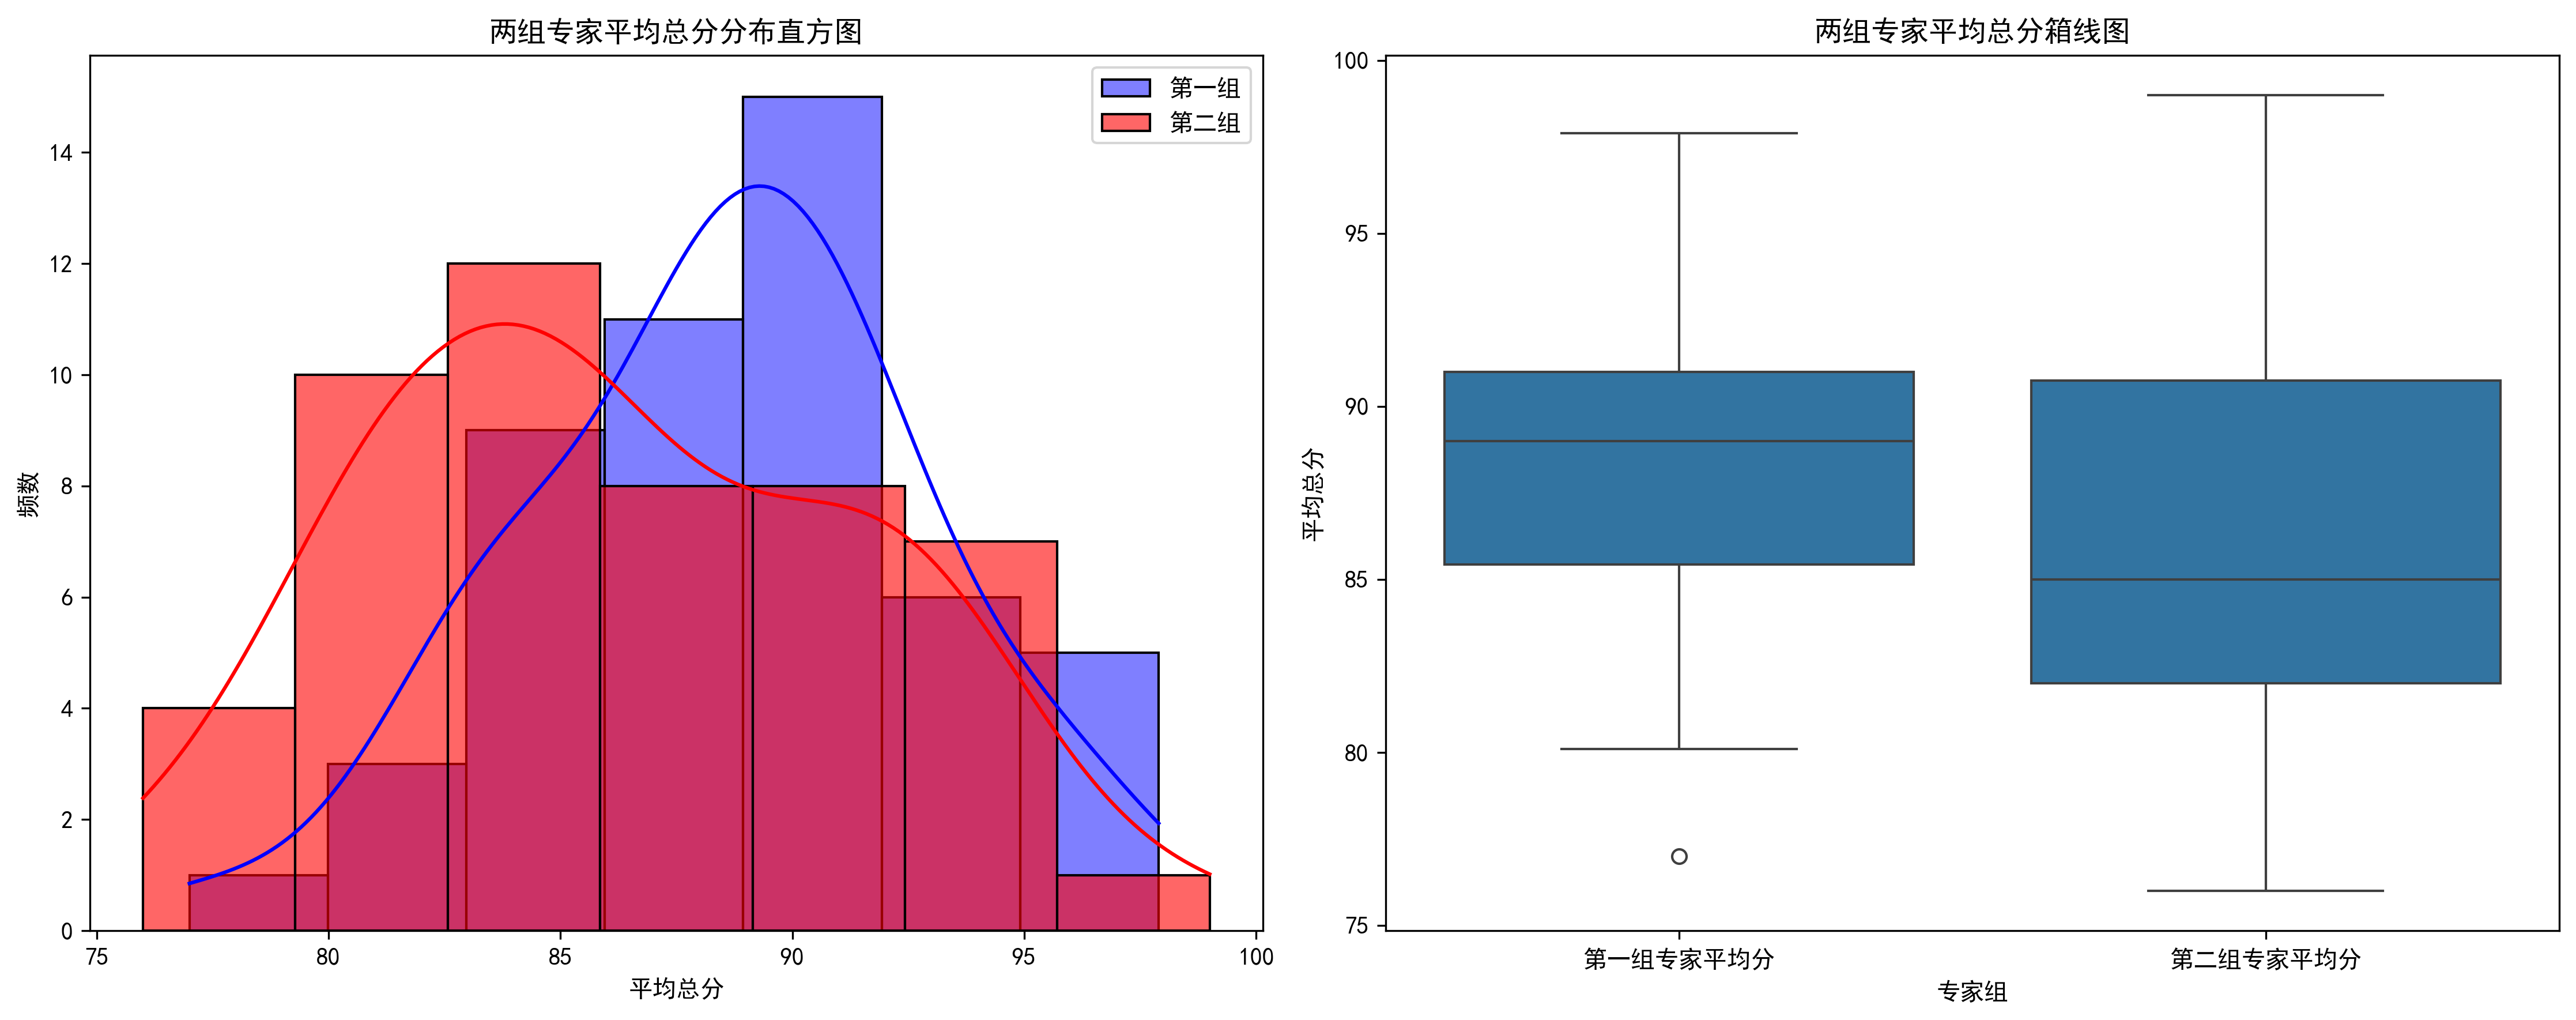
\includegraphics[width=0.75\textwidth]{figures/descriptive_statistics.png}
% \caption{单图}
\label{fig:单图}
\end{figure}

\begin{figure}[ht]
\centering
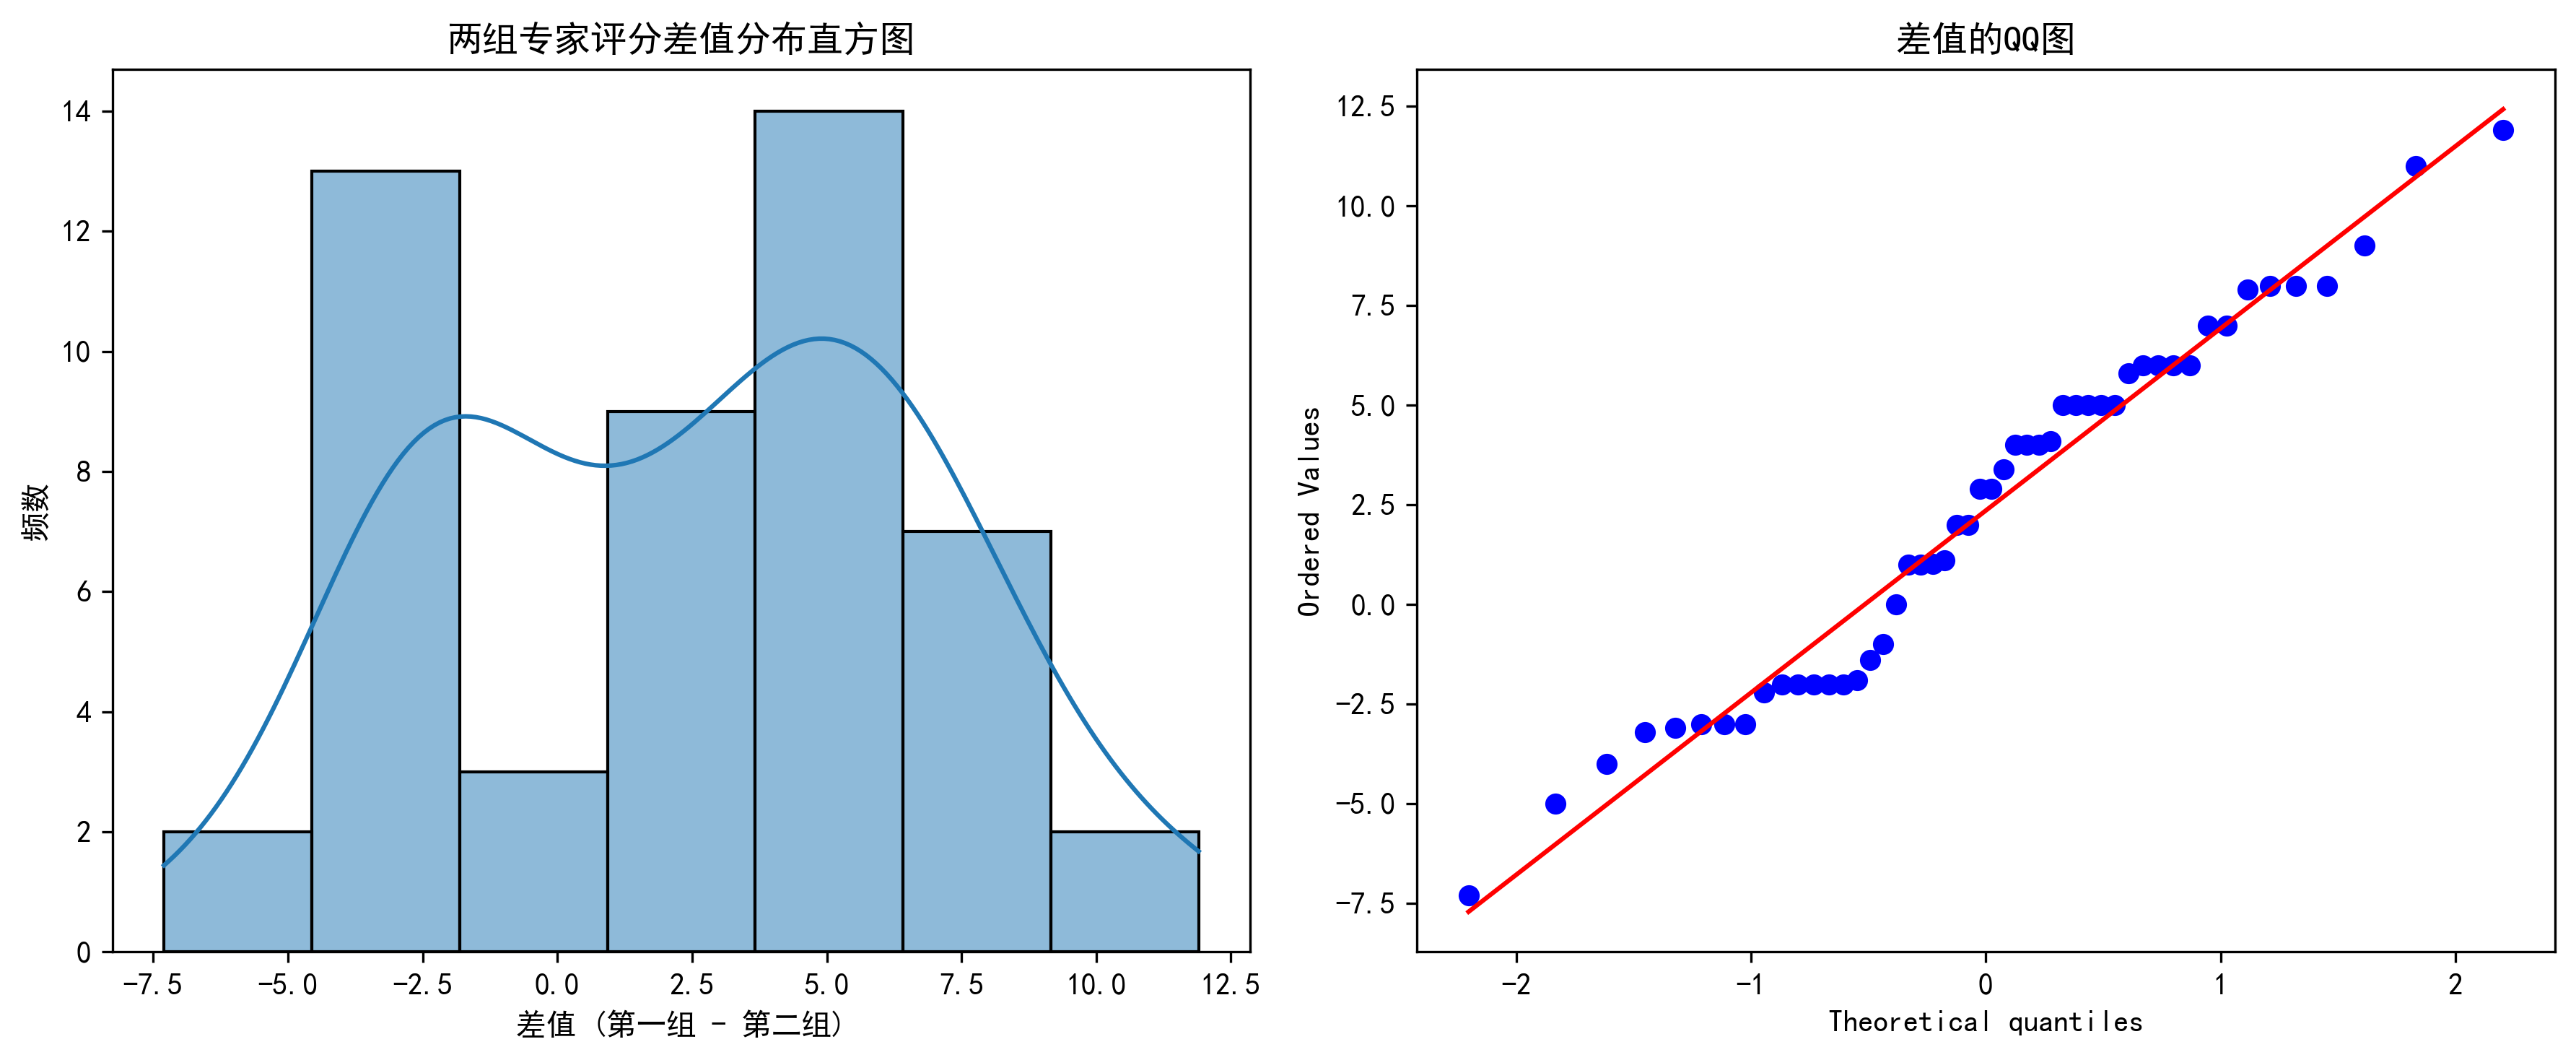
\includegraphics[width=0.75\textwidth]{figures/normality_test.png}
% \caption{单图}
\label{fig:单图}
\end{figure}

\textbf{Step3:} 组内一致性分析,ICC(2,1)结果分别为:第一组$0.518$(中等一致性),第二组$0.323$(较差)。第一组评分标准和稳定性明显优于第二组。


\begin{figure}[H]
\centering
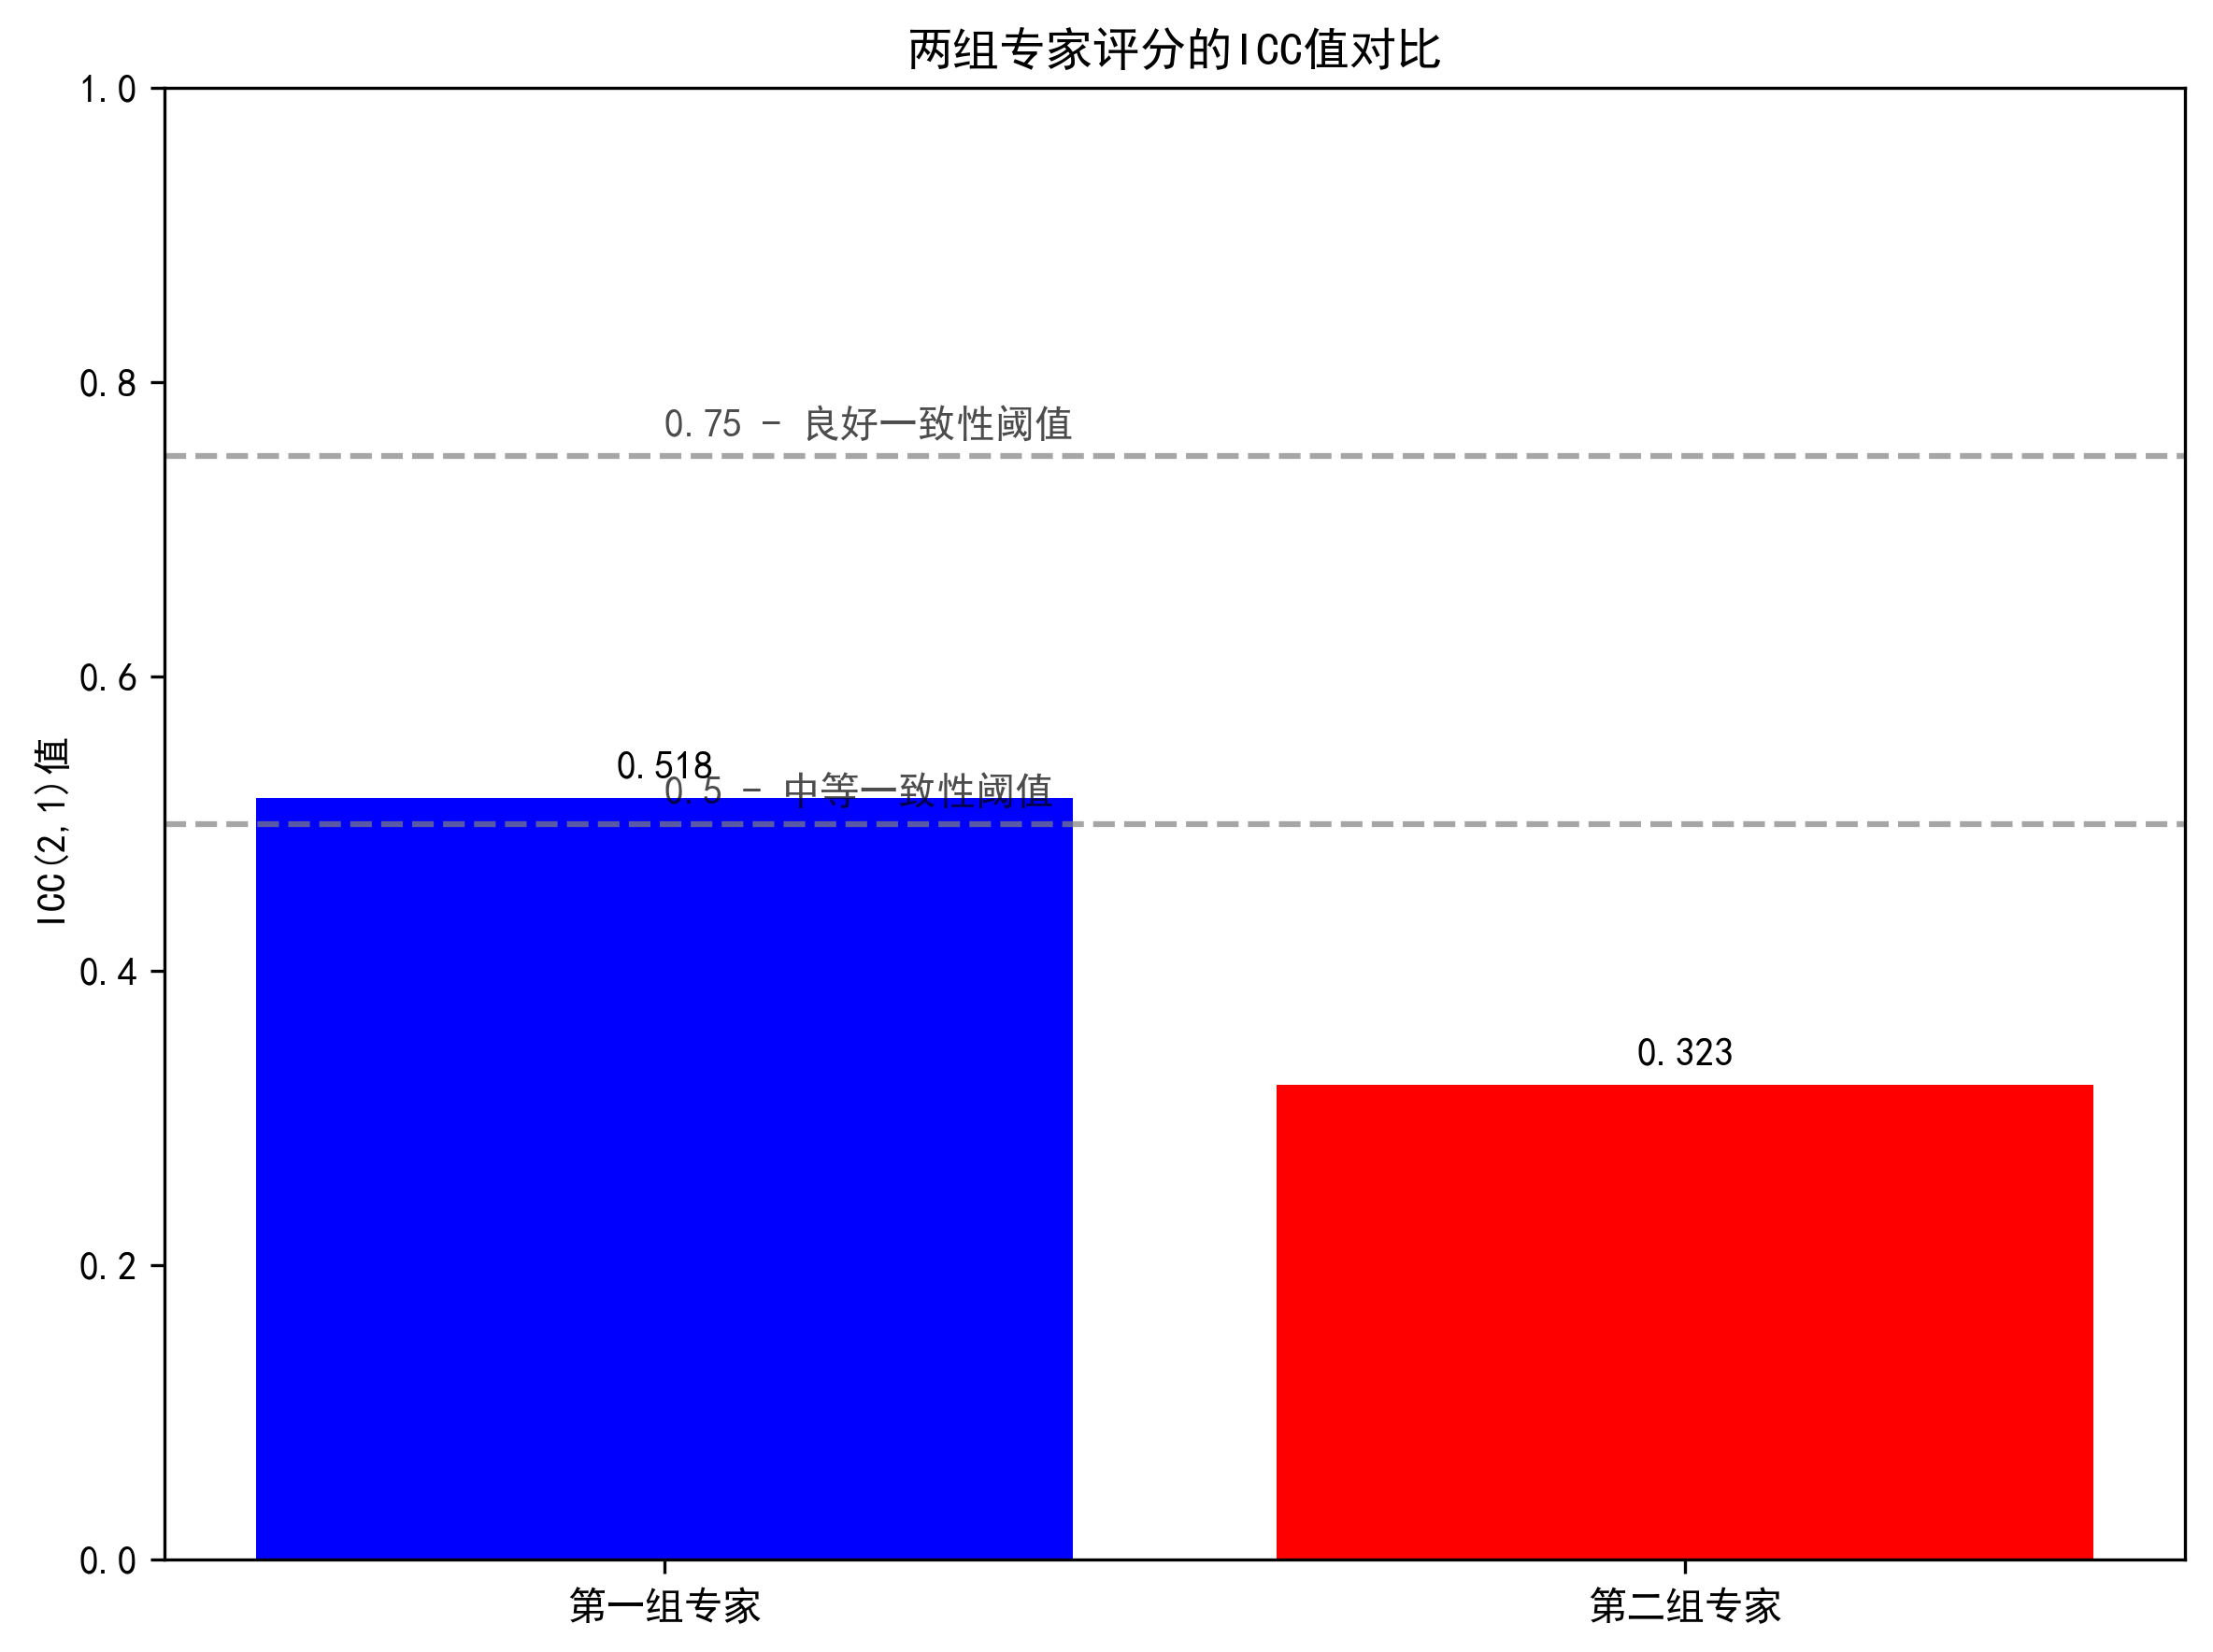
\includegraphics[width=0.75\textwidth]{figures/icc_analysis.png}
% \caption{单图}
\label{fig:单图}
\end{figure}

\subsubsection{求解结果}
综合上述结果,两组专家评分在统计意义上有显著差异,第一组评分一致性更高,更具可信度。在评价体系优化和权重调整时建议优先参考一致性更高的专家组评分。


\section{问题二的模型建立和求解}
\subsection{模型建立}
\textbf{层级贝叶斯模型结构}
分为三层:
\begin{align*}
    S_{ijk} &\sim \mathcal{N}(\mu_{global} + \alpha_i + \beta_{ij},\ \sigma_{error}^2) \\
    \alpha_i &\sim \mathcal{N}(0,\ \sigma_{college}^2) \\
    \beta_{ij} &\sim \mathcal{N}(0,\ \sigma_{expert\_group}^2)
\end{align*}
其中$\sigma_{college}$和$\sigma_{expert\_group}$分别表征学院间、专家组间系统性变异程度。

为直观展示各学院原始分数分布,图\ref{fig:college_scores_boxplot}给出了箱线图。

\begin{figure}[H]
\centering
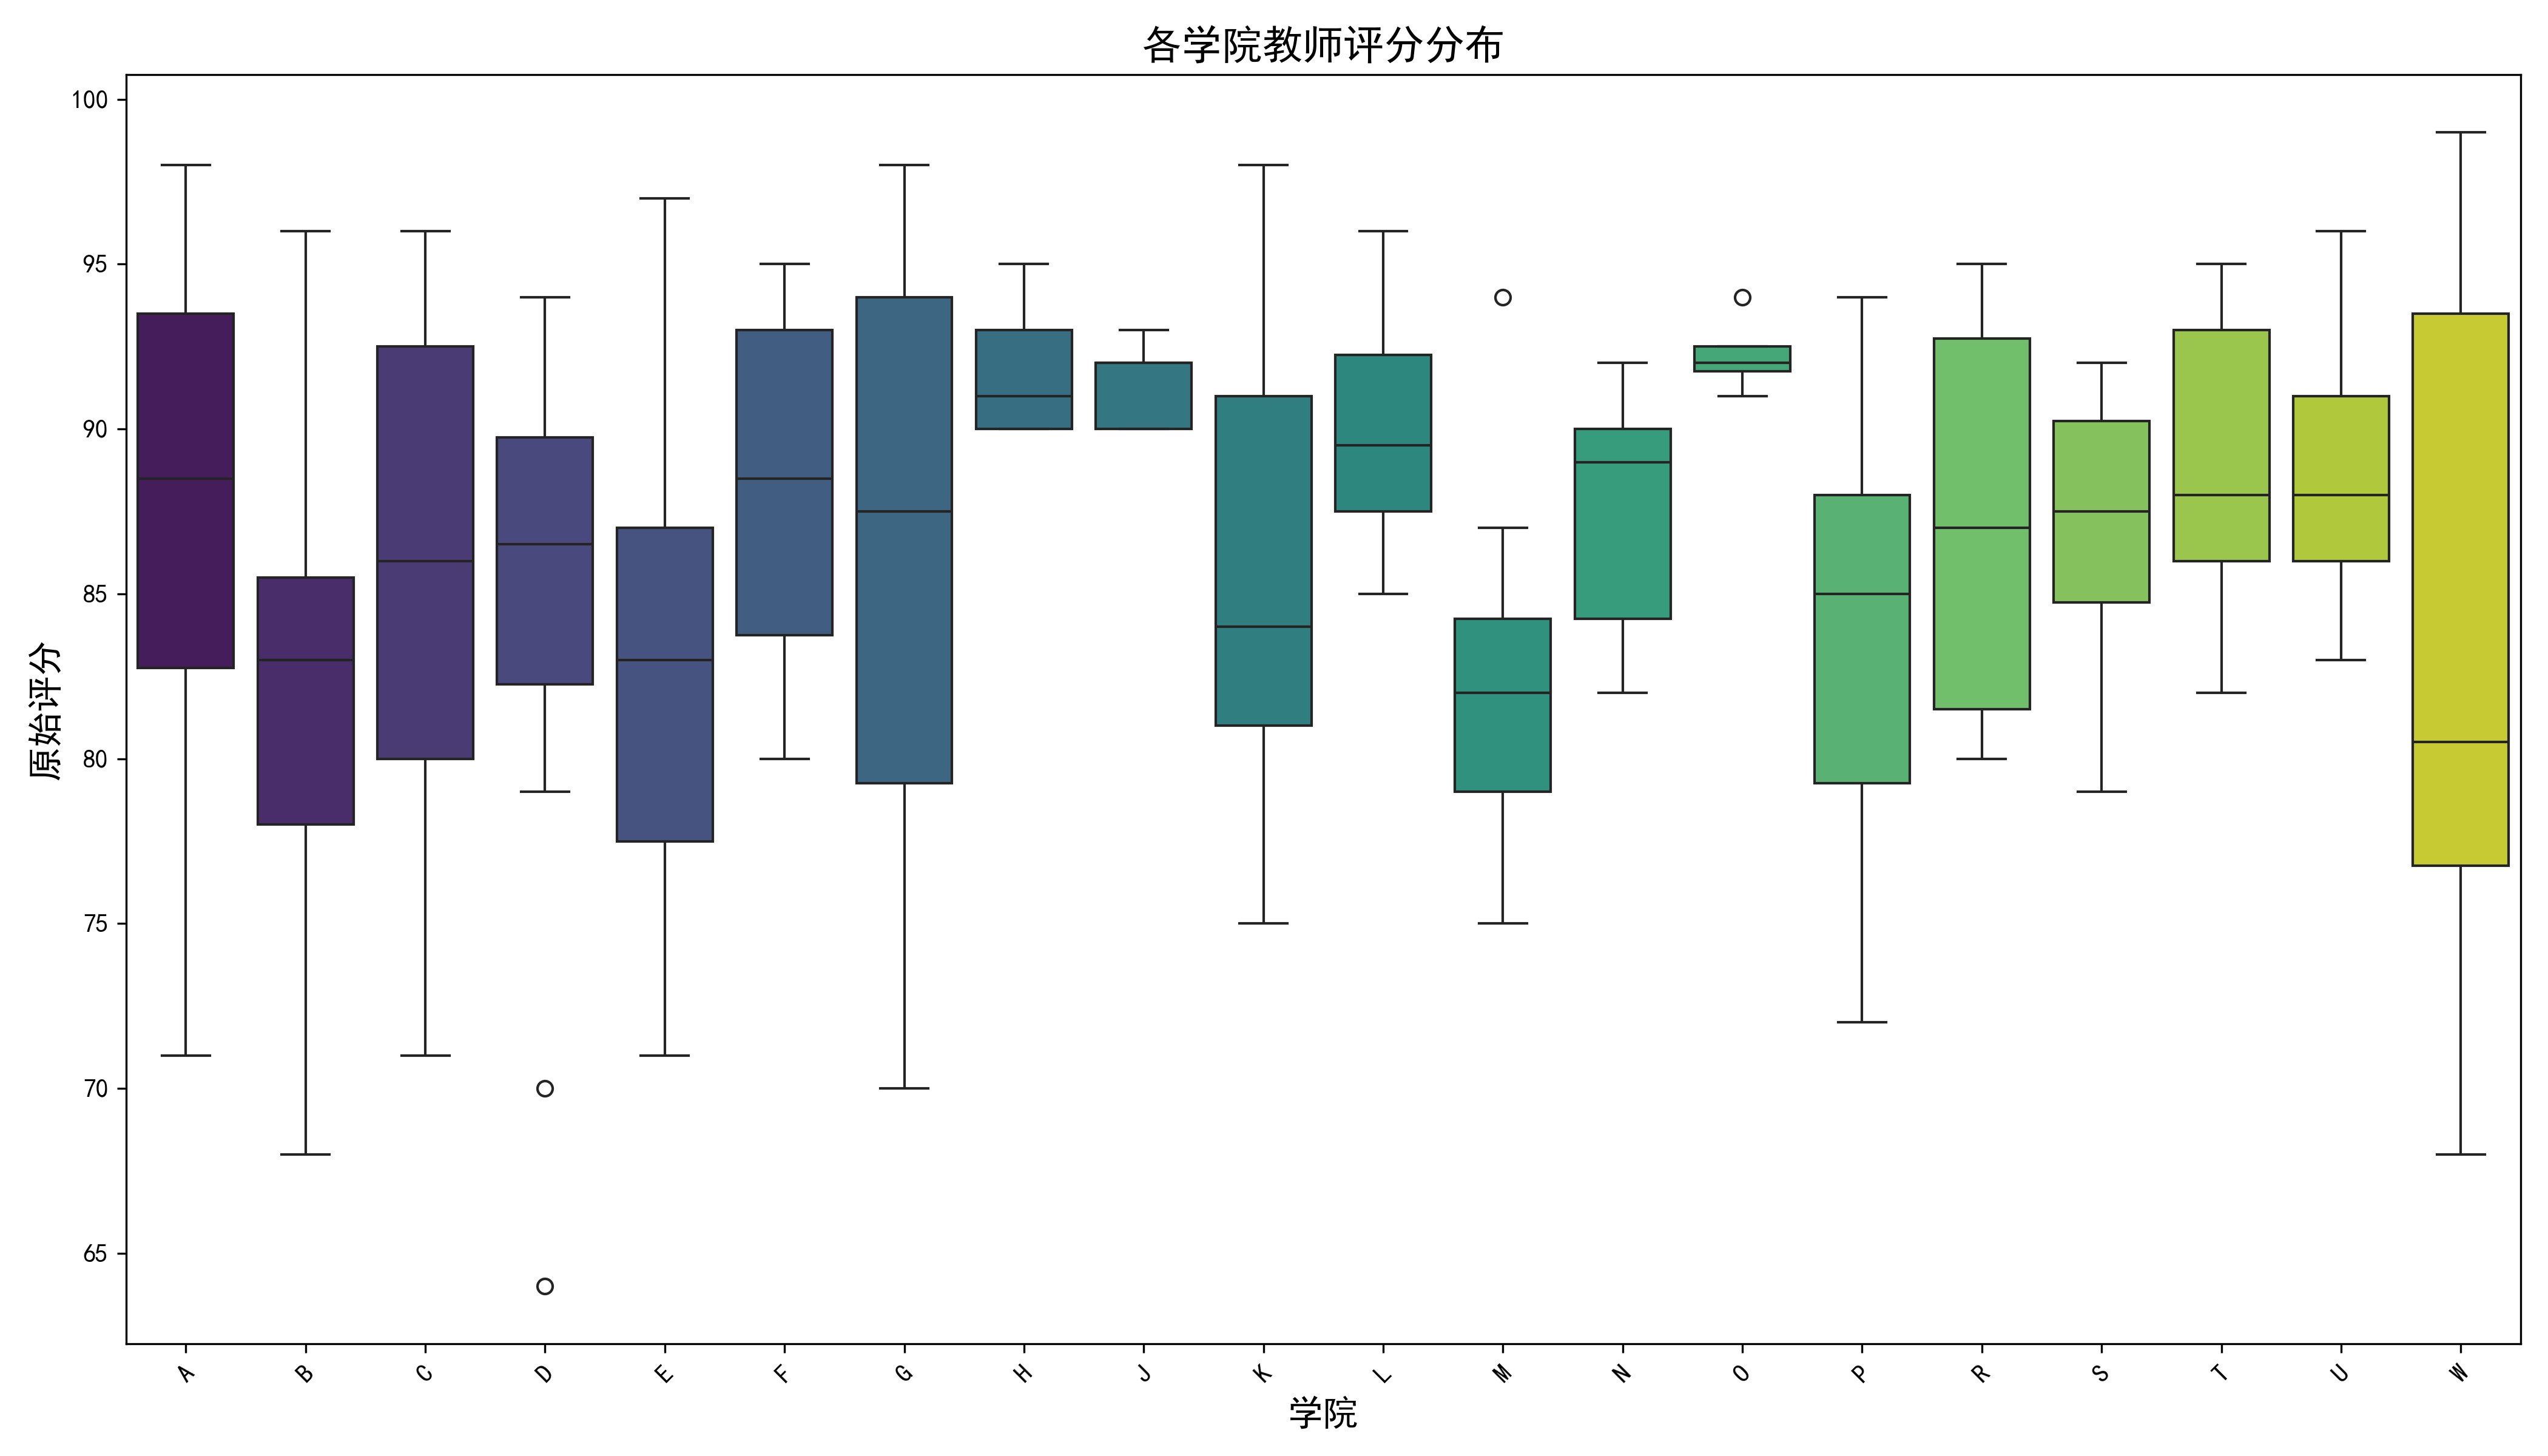
\includegraphics[width=0.75\textwidth]{figures/EDA/college_scores_boxplot.png}
\caption{各学院原始分数分布箱线图}
\label{fig:college_scores_boxplot}
\end{figure}

\textbf{参数先验与贝叶斯推断}
\begin{itemize}
    \item $\mu_{global}$ 选宽阔正态分布为先验,$\sigma_{error},\ \sigma_{college},\ \sigma_{expert\_group}$可选Inverse-Gamma等弱信息先验。
    \item 采用马尔科夫链蒙特卡洛(MCMC)等方法采样后验,实现参数估计与不确定性量化。
\end{itemize}

\subsection{模型求解}
\textbf{Step 1:模型拟合与参数后验估计}
\begin{enumerate}
    \item 整理原始数据$(S_{ijk})$,按“学院-专家组-教师”嵌套输入;
    \item 用Bayesian工具(如PyMC3、Stan等)编码上述分层模型,设定先验;
    \item 运行MCMC,检查traceplot与Rhat指标,确保收敛,获取各层次效应的后验分布和均值估计;
    \item 计算$\widehat{\mu}_{global}$、$\widehat{\alpha}_{i}$、$\widehat{\beta}_{ij}$并保存。
\end{enumerate}

模型参数采样的后验分布如图\ref{fig:posterior_plots}所示,采样过程的收敛性见图\ref{fig:trace_plots}。

\begin{figure}[H]
\centering
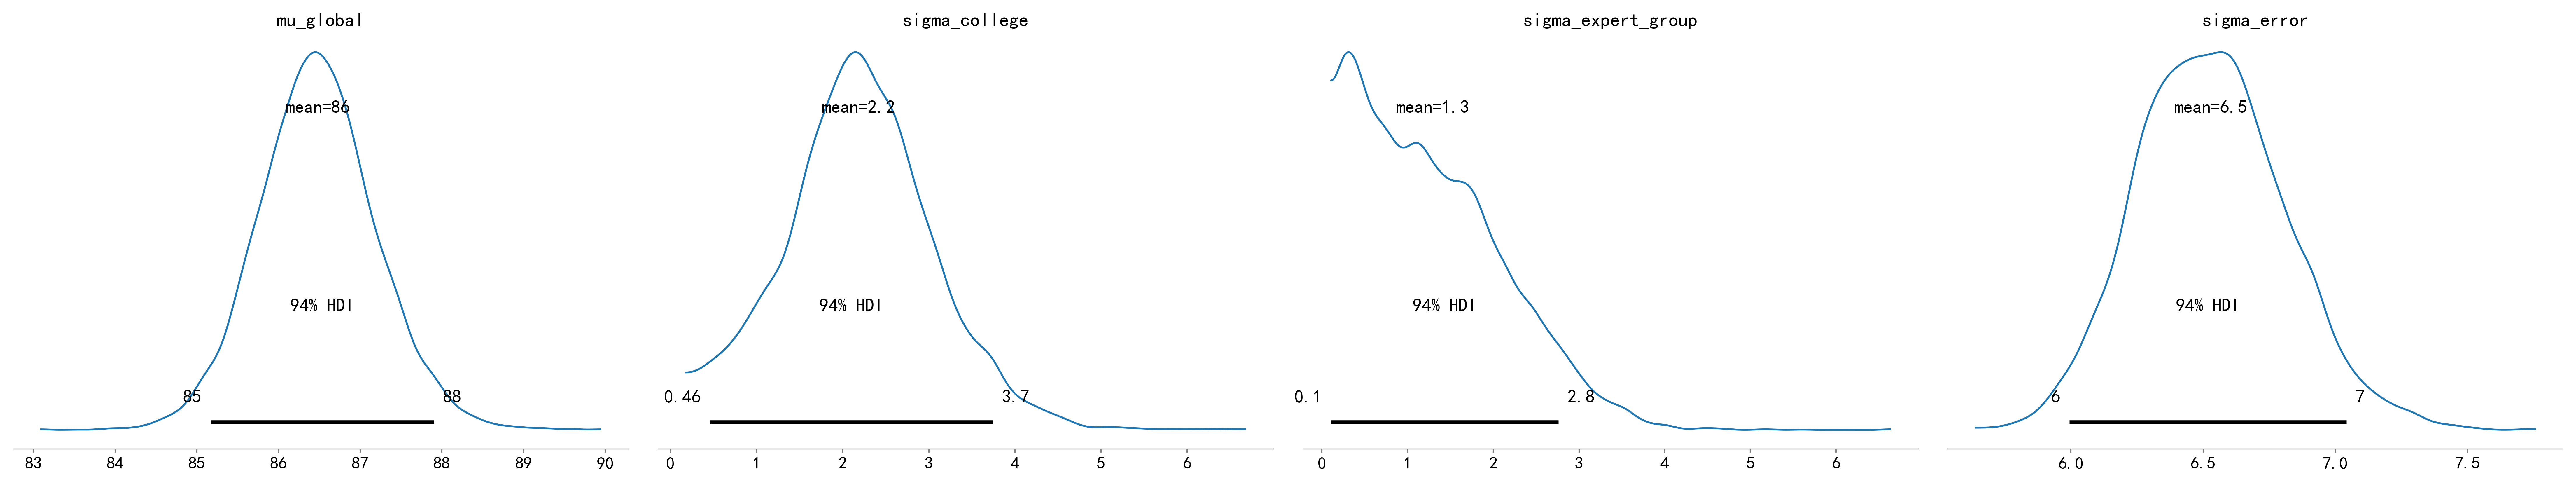
\includegraphics[width=1\textwidth]{figures/Diagnostics/posterior_plots.png}
\caption{主要参数后验分布图}
\label{fig:posterior_plots}
\end{figure}

\begin{figure}[H]
\centering
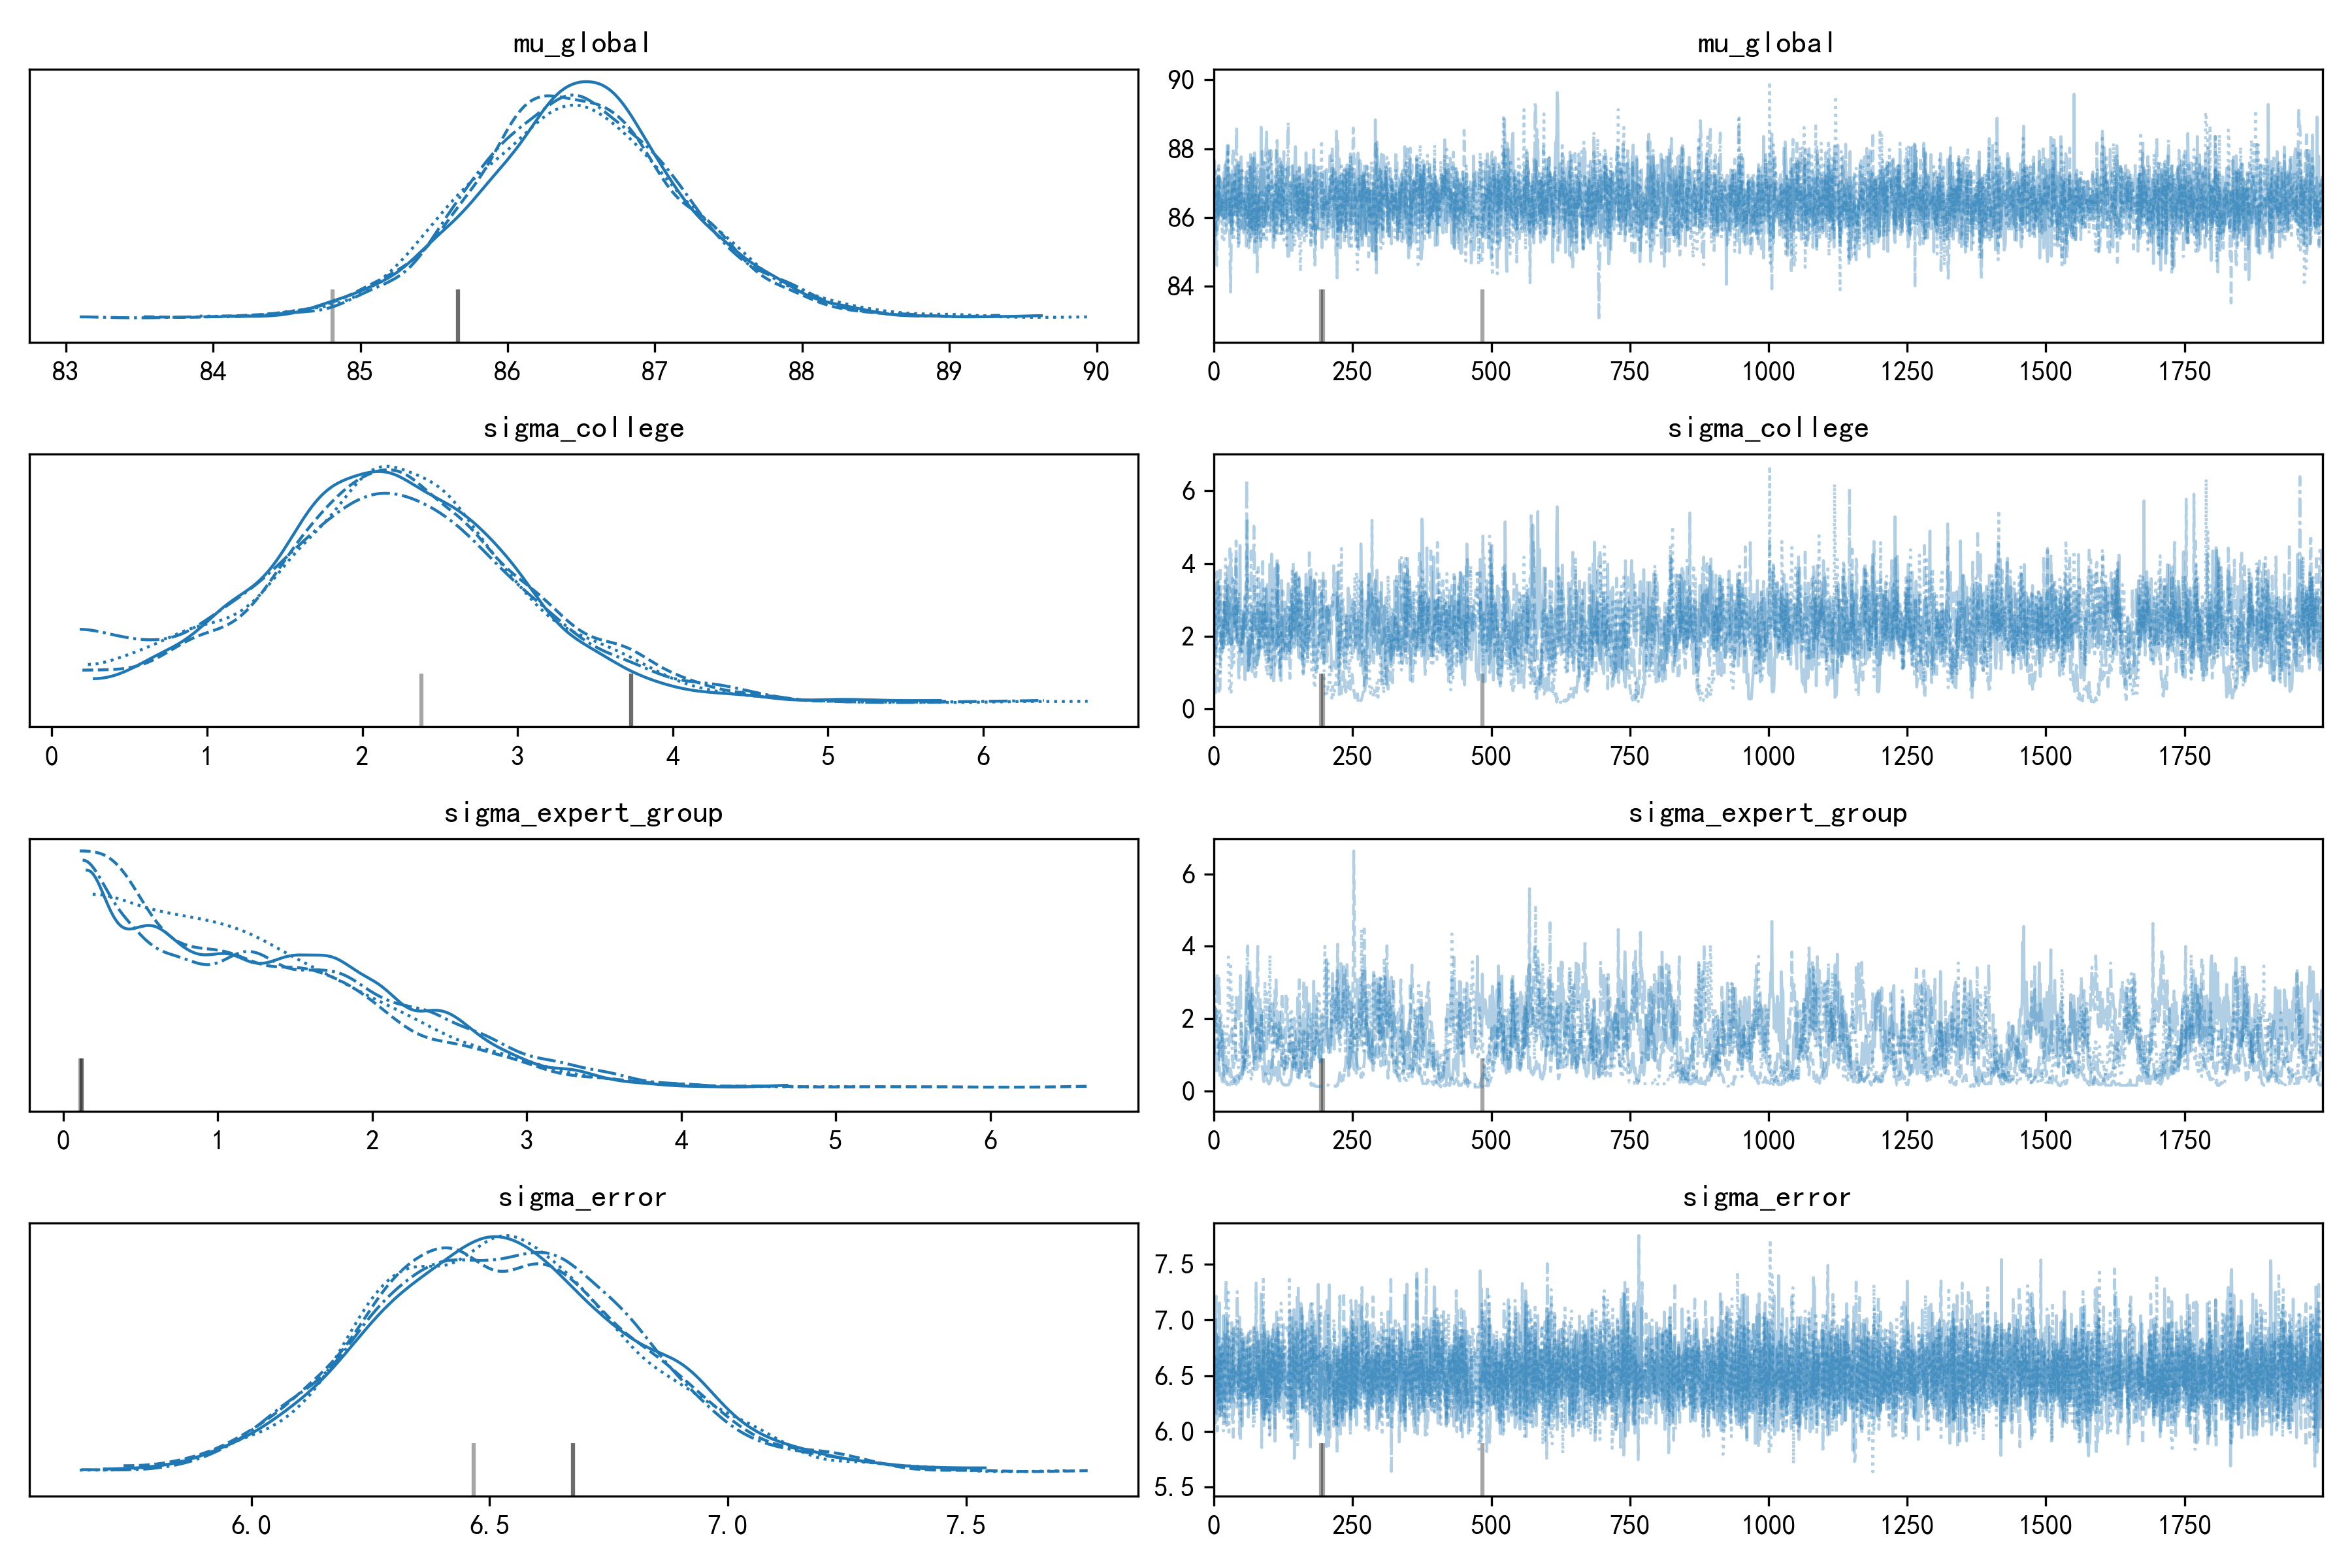
\includegraphics[width=1\textwidth]{figures/Diagnostics/trace_plots.png}
\caption{MCMC采样traceplot诊断图}
\label{fig:trace_plots}
\end{figure}

\textbf{Step 2:系统性偏差校正与分数标准化}
\begin{itemize}
    \item 对每一位教师的得分$S_{ijk}$,计算剥离偏差后的校正分数:
    $$
    \widetilde{S}_{ijk} = S_{ijk} - \widehat{\alpha}_i - \widehat{\beta}_{ij} + \widehat{\mu}_{global}
    $$
    \item 再对校正分进行标准化映射,使全校分数均值定为85、标准差为5(限制在$[60,100]$区间):
    $$
    S_{final} = \min \left\{100,\ \max\left[60,\ 85 + 5 \times \frac{\widetilde{S}_{ijk} - \overline{\widetilde{S}}}{\widehat{\sigma}_{\widetilde{S}}}\right]\right\}
    $$
    其中$\overline{\widetilde{S}}$为所有校正分均值,$\widehat{\sigma}_{\widetilde{S}}$为标准差。
\end{itemize}

\textbf{Step 3:结果分析与可视化}
校正前后各学院的均值、极差和分布特征变化见图\ref{fig:college_scores_comparison},标准化后分布更加集中,极端差异明显减小。

\begin{figure}[H]
\centering
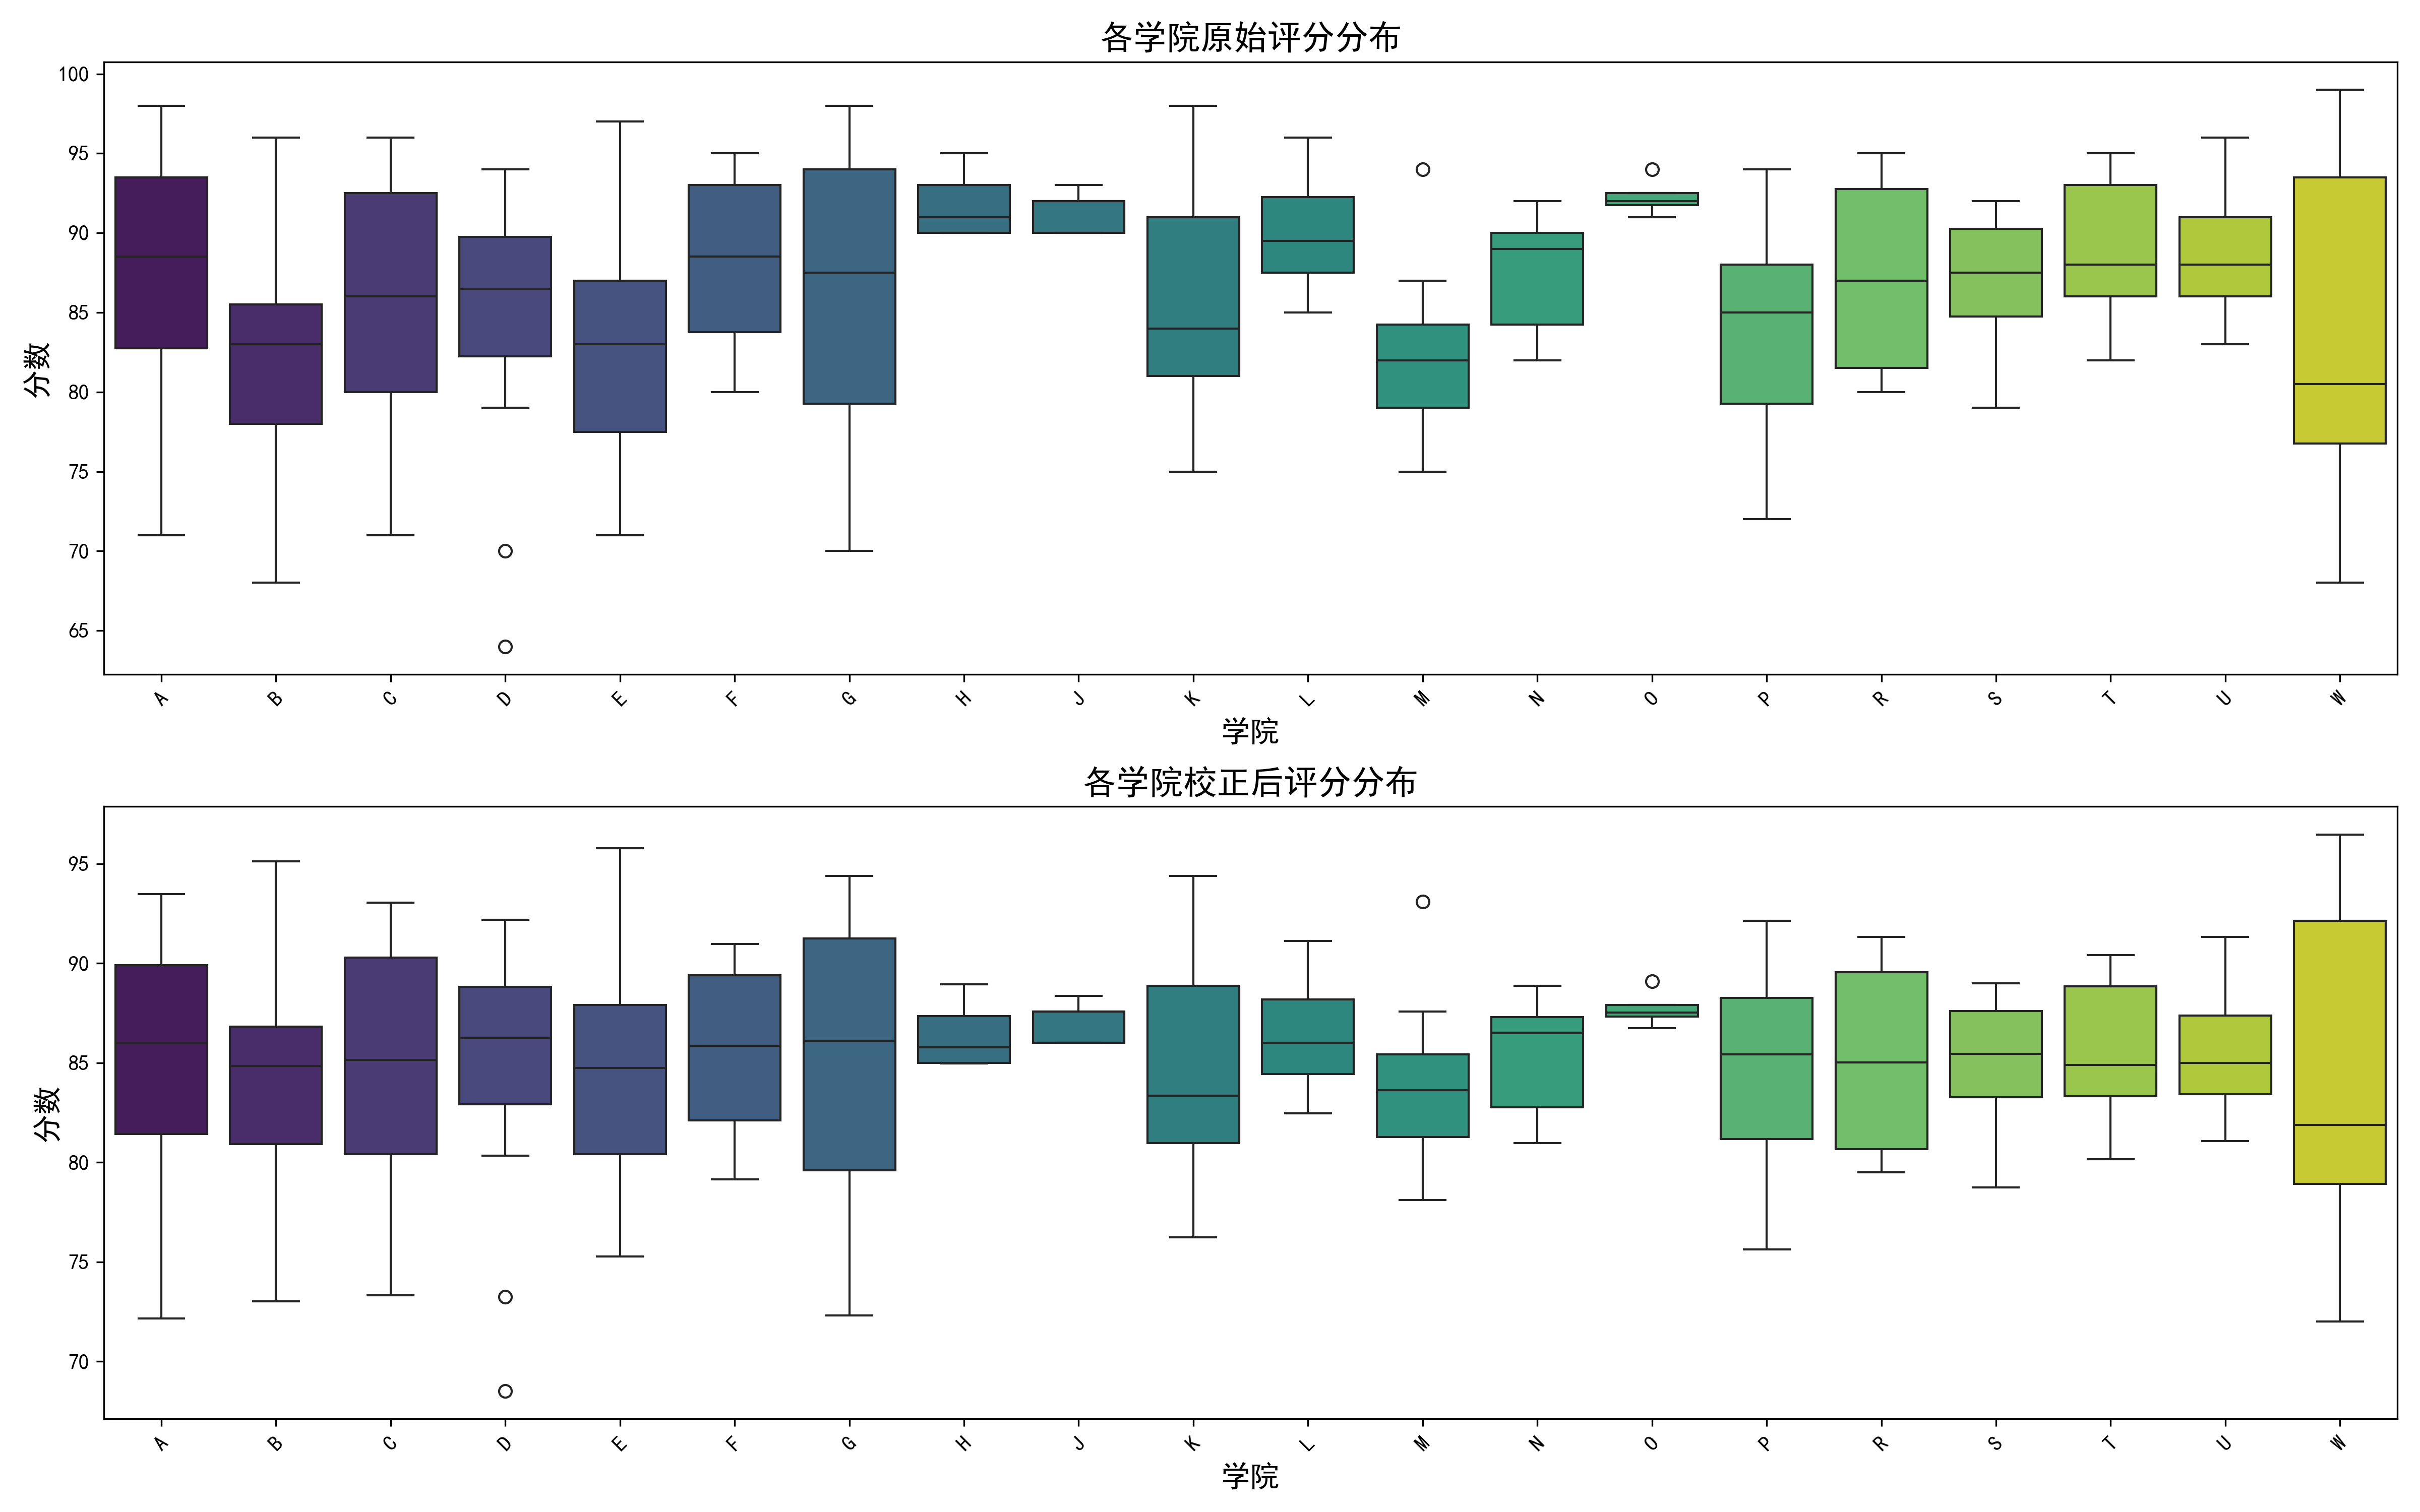
\includegraphics[width=1\textwidth]{figures/Results_Visualization/college_scores_comparison.png}
\caption{校正前后各学院分数分布对比}
\label{fig:college_scores_comparison}
\end{figure}

教师排名和分数分布的变化见图\ref{fig:rank_comparison_scatter}和图\ref{fig:score_distributions_comparison},可以看出模型提升了整体的公平性。

\begin{figure}[H]
\centering
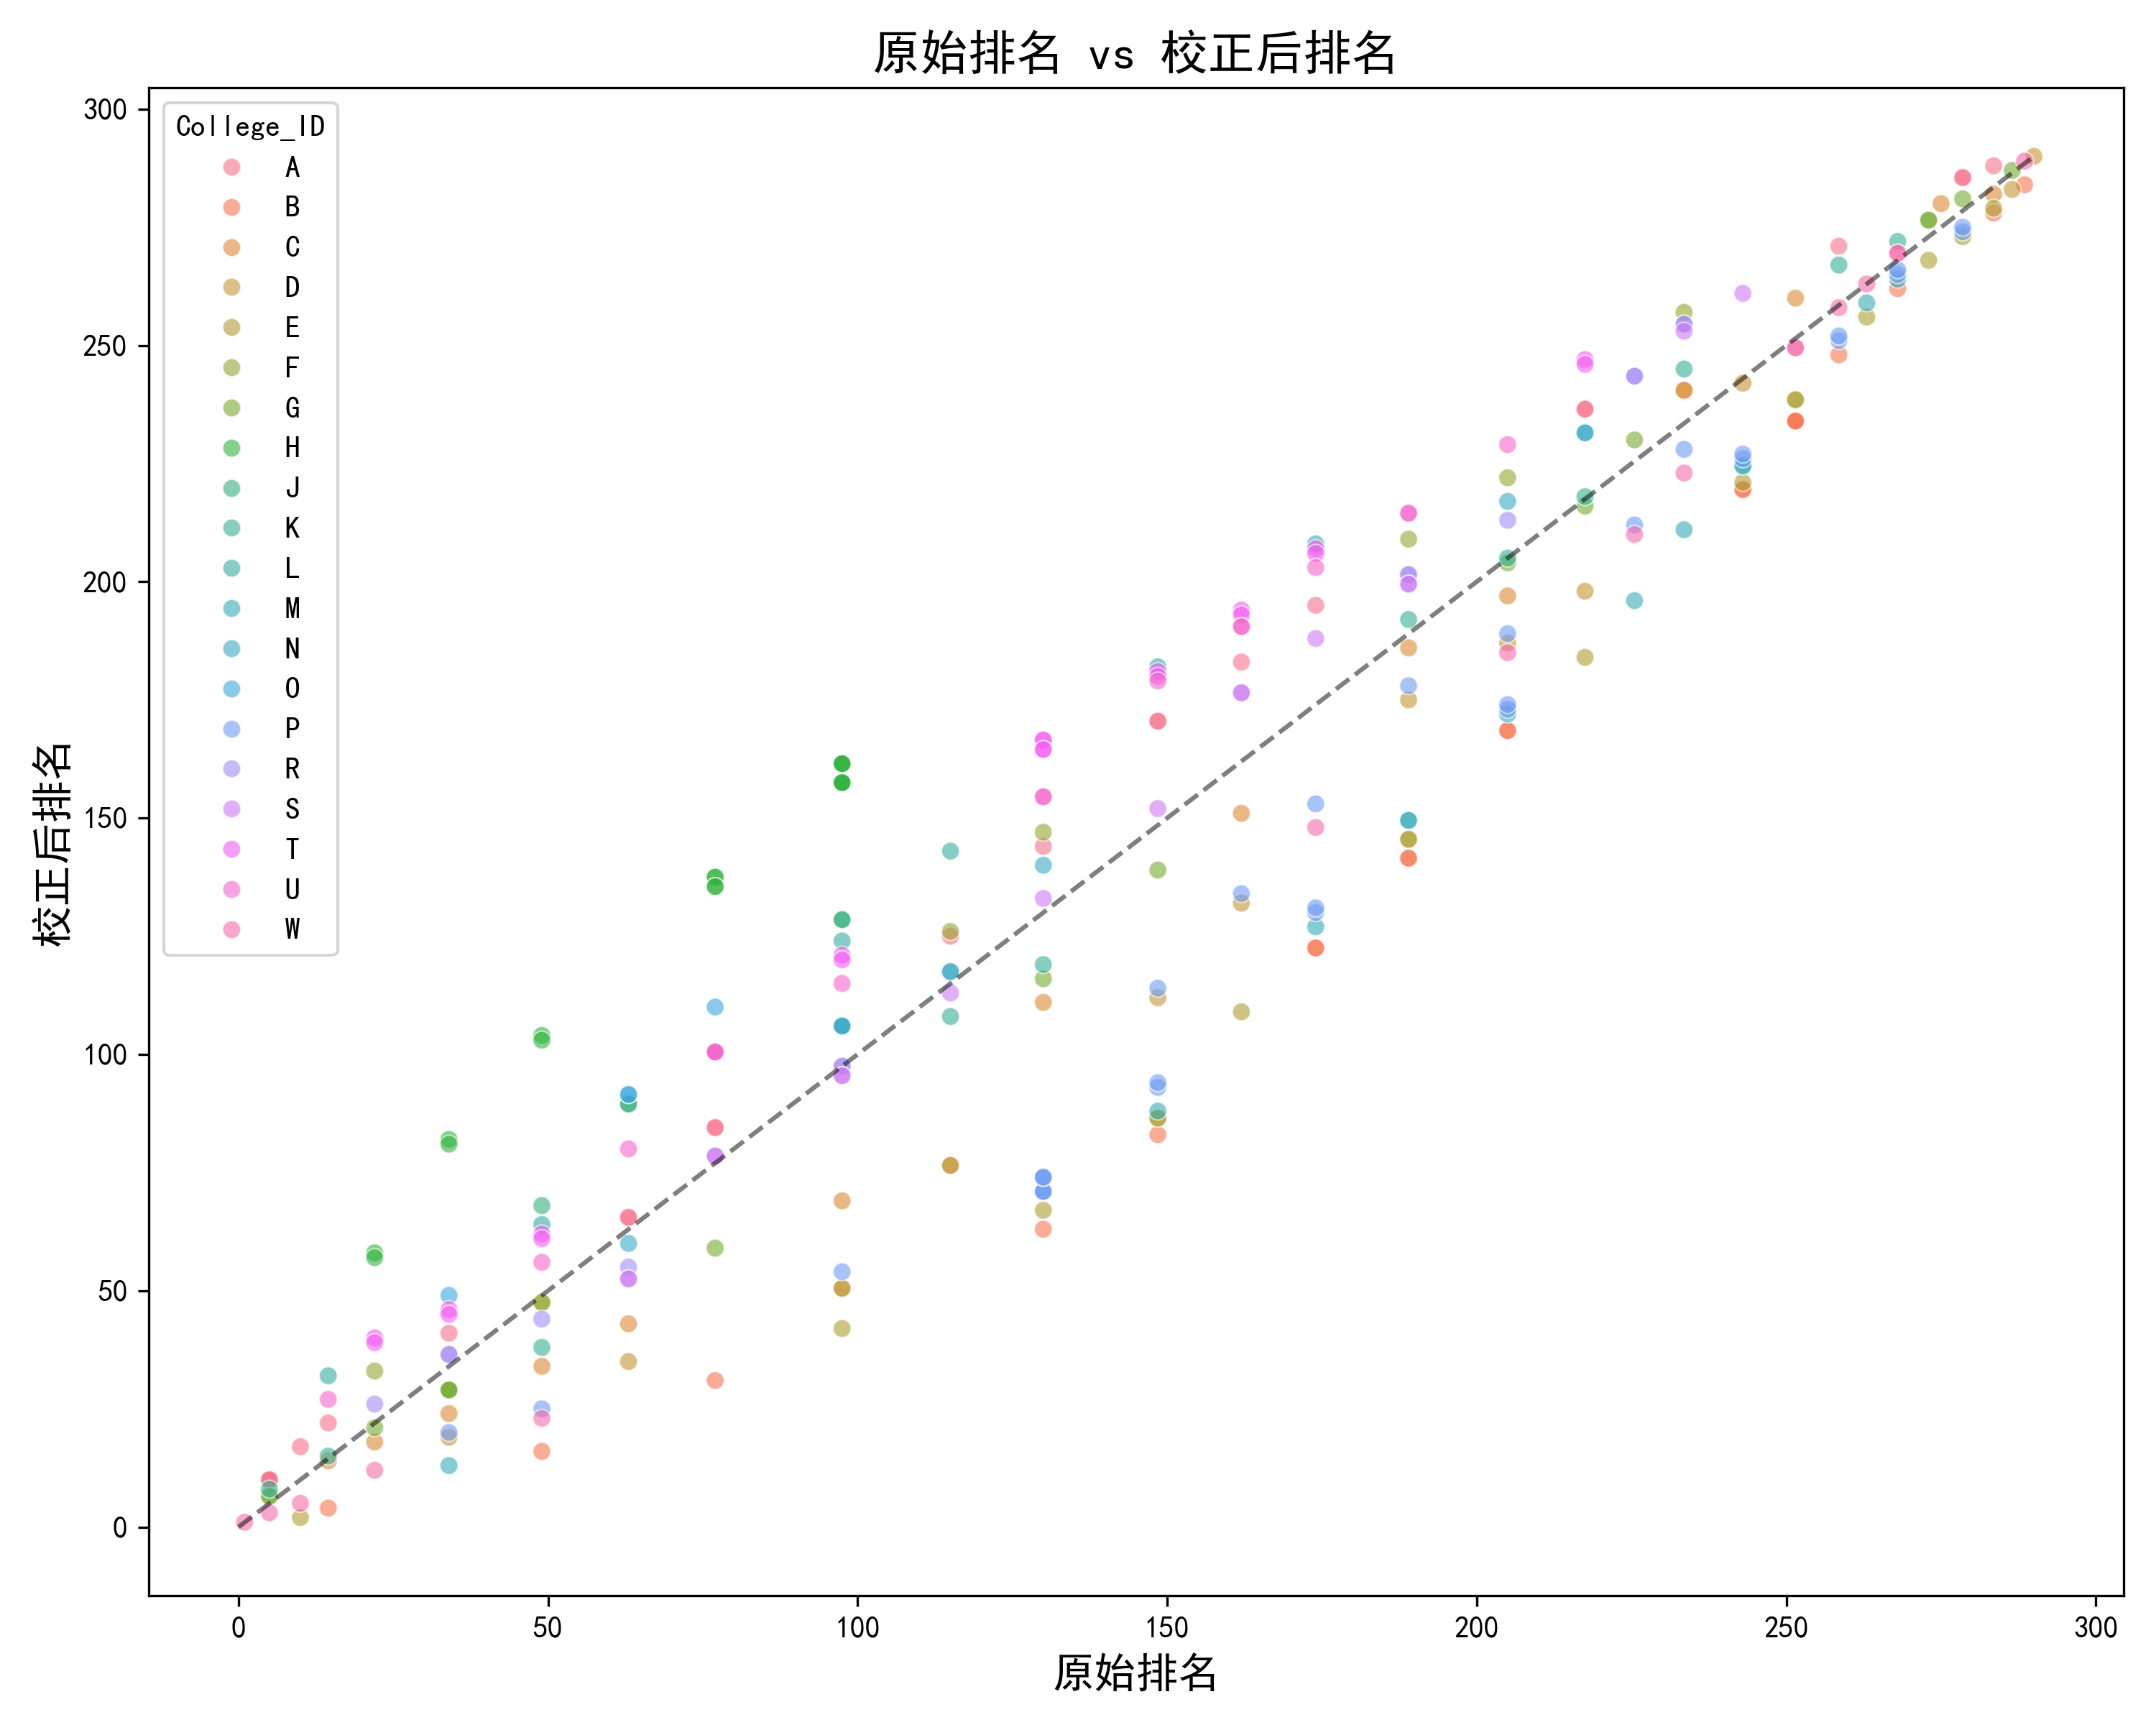
\includegraphics[width=1\textwidth]{figures/Results_Visualization/rank_comparison_scatter.png}
\caption{校正前后教师排名变化散点图}
\label{fig:rank_comparison_scatter}
\end{figure}

\begin{figure}[H]
\centering
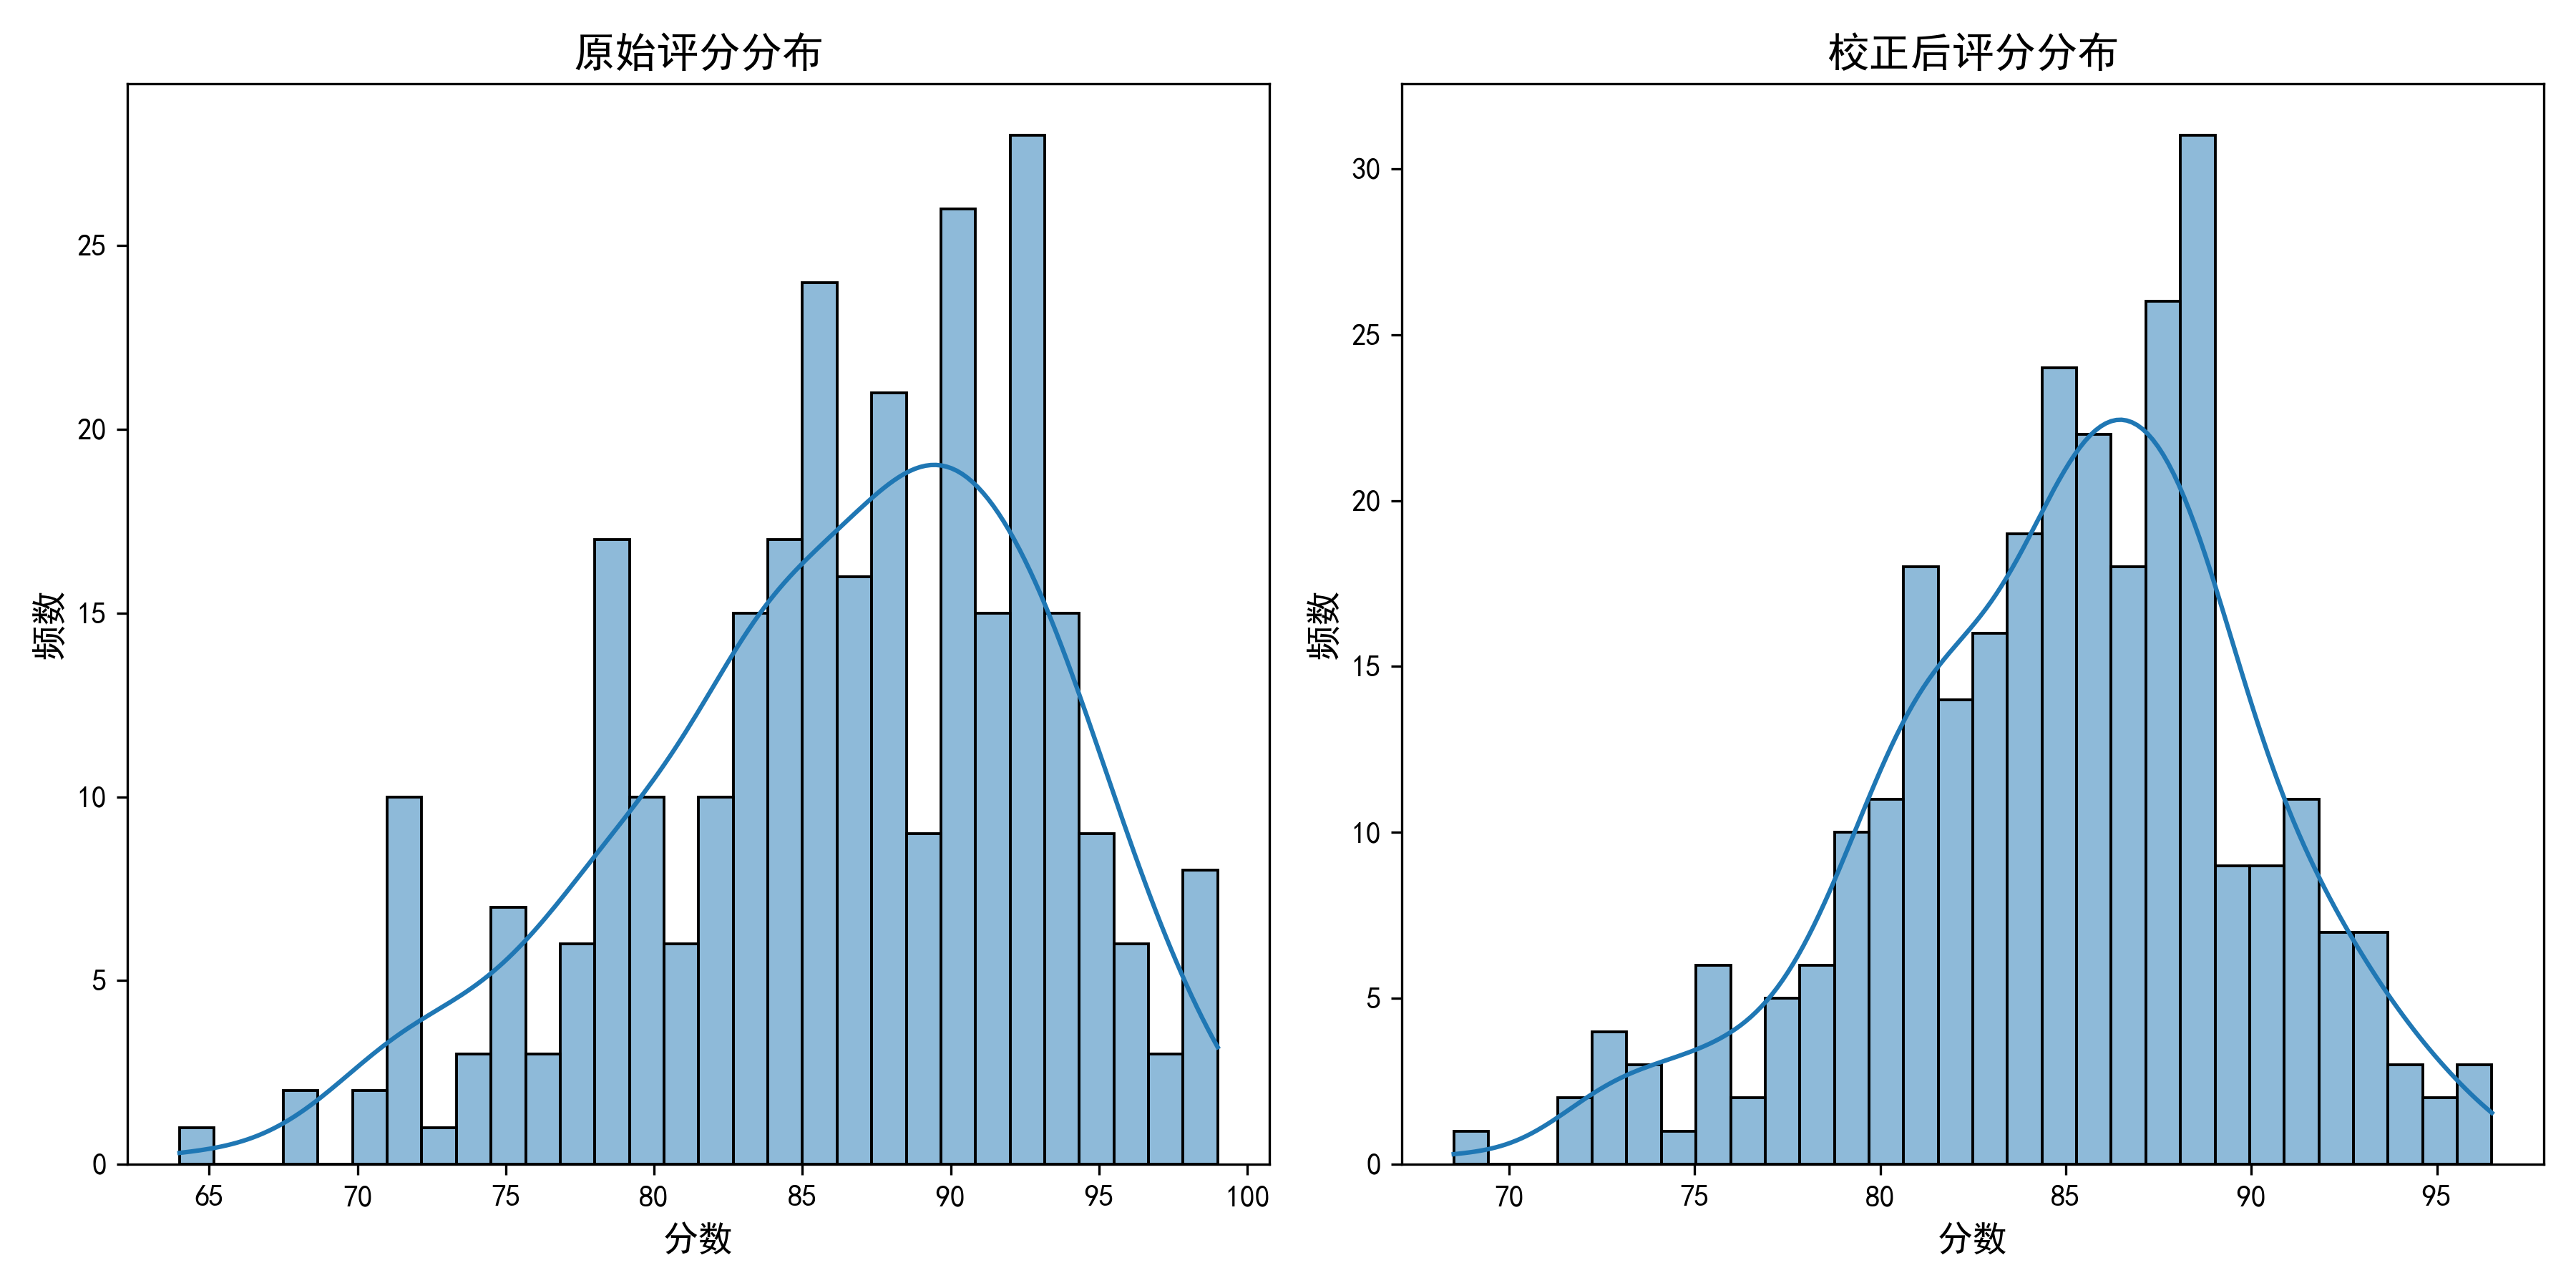
\includegraphics[width=1\textwidth]{figures/Results_Visualization/score_distributions_comparison.png}
\caption{分数分布直方图对比,校正后分布更接近正态}
\label{fig:score_distributions_comparison}
\end{figure}



\section{问题二的模型的建立和求解}
\subsection{模型建立}

引用\cref{fig:双图},引用\cref{fig:双图a},引用\cref{fig:双图b}。

\begin{figure}[ht]
\centering
\subcaptionbox{双图a子标题\label{fig:双图a}}
{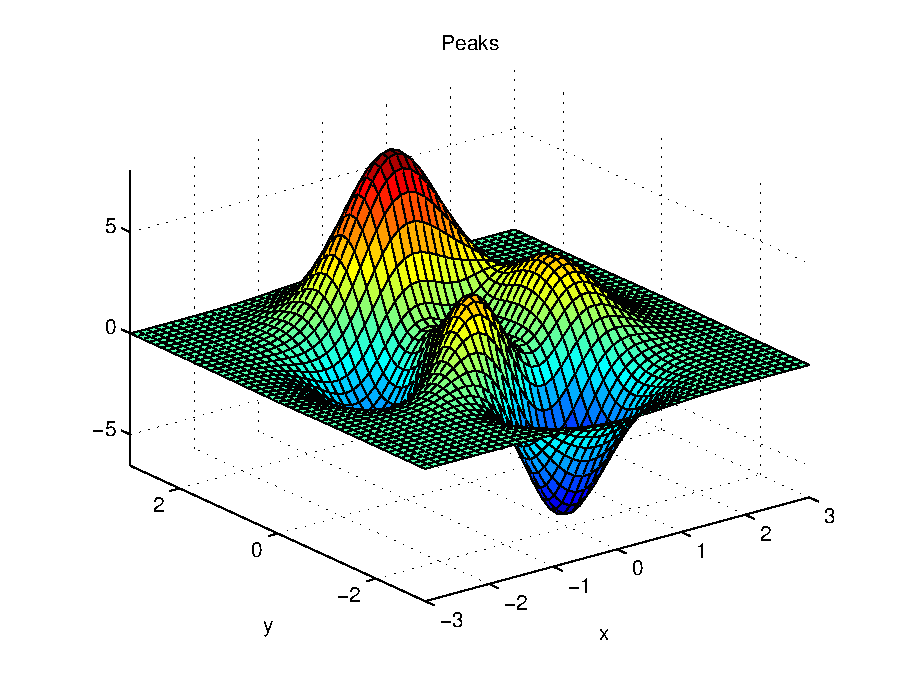
\includegraphics[width=.4\textwidth]{example.eps}}
\subcaptionbox{双图b子标题\label{fig:双图b}}
{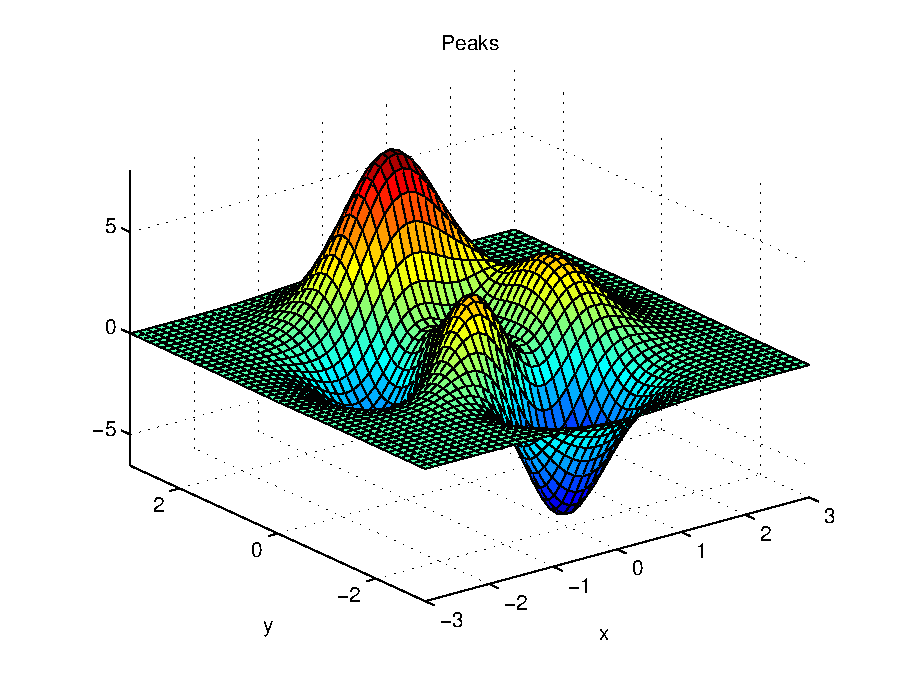
\includegraphics[width=.4\textwidth]{example.eps}}
\caption{双图}\label{fig:双图}
\end{figure} 

\subsection{模型求解}

\textbf{Step1:} 

\textbf{Step2:} 

\textbf{Step3:} 

\subsection{求解结果}

%%%%%%%%%%%%%%%%%%%%%%%%%%%%%%%%%%%%%%%%%%%%%%%%%%%%%%%%%%%%% 

\section{问题三的模型的建立和求解}
\subsection{模型建立}

\subsection{模型求解}

\textbf{Step1:} 

\textbf{Step2:} 

\textbf{Step3:} 

\subsection{求解结果}

%%%%%%%%%%%%%%%%%%%%%%%%%%%%%%%%%%%%%%%%%%%%%%%%%%%%%%%%%%%%% 

\section{问题四的模型的建立和求解}
\subsection{模型建立}

\subsection{模型求解}

\textbf{Step1:} 

\textbf{Step2:} 

\textbf{Step3:} 

\subsection{求解结果}

%%%%%%%%%%%%%%%%%%%%%%%%%%%%%%%%%%%%%%%%%%%%%%%%%%%%%%%%%%%%%

\section{模型的分析与检验}

\subsection{灵敏度分析}

\subsection{误差分析}

%%%%%%%%%%%%%%%%%%%%%%%%%%%%%%%%%%%%%%%%%%%%%%%%%%%%%%%%%%%%%

\section{模型的评价}

\subsection{模型的优点}
\begin{itemize}[itemindent=2em]
\item 优点1
\item 优点2
\item 优点3
\end{itemize}

\subsection{模型的缺点}
\begin{itemize}[itemindent=2em]
\item 缺点1
\item 缺点2
\end{itemize}

%%%%%%%%%%%%%%%%%%%%%%%%%%%%%%%%%%%%%%%%%%%%%%%%%%%%%%%%%%%%%
%% 参考文献
\nocite{*}
\bibliographystyle{gbt7714-numerical}  % 引用格式
\bibliography{ref.bib}  % bib源

\newpage
%%%%%%%%%%%%%%%%%%%%%%%%%%%%%%%%%%%%%%%%%%%%%%%%%%%%%%%%%%%%%
%% 附录
\begin{appendices}
\section{文件列表}
\begin{table}[H]
\centering
\begin{tabularx}{\textwidth}{LL}
\toprule
文件名   & 功能描述 \\
\midrule
q1.m & 问题一程序代码 \\
q2.py & 问题二程序代码 \\
q3.c & 问题三程序代码 \\
q4.cpp & 问题四程序代码 \\
\bottomrule
\end{tabularx}
\label{tab:文件列表}
\end{table}

\section{代码}
\noindent q1.m
\lstinputlisting[language=matlab]{code/q1.m}
q2.py
\lstinputlisting[language=python]{code/q2.py}
q3.c
\lstinputlisting[language=c]{code/q3.c}
q4.cpp
\lstinputlisting[language=c++]{code/q4.cpp}
\end{appendices}
\end{document}


%%%%%双图模板%%%%%%
\begin{figure}
\centering
\subcaptionbox{炉温曲线示意图\label{fig:双图a}}
{\includegraphics[width=.4\textwidth]{炉温曲线示意图.png}}
\subcaptionbox{问题1炉温曲线\label{fig:双图b}}
{\includegraphics[width=.4\textwidth]{问题1炉温曲线.png}}
\caption{双图}\label{fig:双图}
\end{figure} 
%%%%%双图模板%%%%%%